\chapter[Search for high mass resonances decaying to a W boson pair with first \boldmath$13\TeV$ data]{Search for high mass resonances decaying to a W boson pair with first 13\TeV data}\label{chap6}
\chaptermark{Search for high mass resonances decaying to a W boson pair at \boldmath$13\TeV$}
\thispagestyle{empty}

In this chapter, a search for a high mass spin-0 particle (from now on denoted as X) in the $\mathrm{X\to WW \to e^{\pm}\mu^{\mp}\nu\bar{\nu}}$ decay channel is presented. 
The search is based upon the same proton-proton collision data samples considered in the previous chapter, corresponding to an integrated luminosity of 2.3\ifb  at $\sqrt{s} = 13$\TeV. This analysis represents a general extension of the SM Higgs boson measurement presented in Chapter~\ref{chap5} and is performed in a range of heavy scalar masses from $M_\mathrm{X} = 200$\GeV up to 1\TeV, extending the range studied in a similar analysis performed using Run 1 LHC data~\cite{Khachatryan:2015cwa}, which provided upper limits on the production cross section of new scalar resonances up to 600\GeV.

%Despite the discovery of a particle consistent with the SM Higgs boson in 2012, there is a possibility that this particle is only a part of a larger Higgs sector, and hence only partially responsible of the EW symmetry breaking. This can be achieved in different theoretical models that extends the SM, such as the two-Higgs-doublet models~\cite{Branco:2011iw,craig,Haber:2015}, or models in which the SM Higgs boson mixes with a heavy EW singlet, which predict the existence of an additional resonance at high mass, with couplings similar to those of the SM Higgs boson, as most recently described in~\cite{Chpoi:2013wga,Robens:2015gla}.

This analysis reports a generic search for a scalar particle assuming different decay width hypotheses, produced via the ggH and VBF production mechanisms. The results can then be interpreted in terms of different theoretical models, such as the ones discussed in Sec.~\ref{sec:BSM}. This analysis is based on the SM Higgs boson measurement described in Chapter~\ref{chap5} in terms of physics objects, selections and background estimations. The differences are discussed in the following sections.

%\section{Introduction}\label{chap6:introduction}

In this chapter, a search for a high mass spin-0 particle (from now on denoted as X) in the X$\rightarrow$WW$\rightarrow \ell\nu\ell'\nu'$ decay channel is presented, where $\ell$ and $\ell'$ refer to an different flavour lepton pair, i.e. e$\mu$. 
The search is based upon proton-proton collision data samples corresponding to an integrated luminosity
of up to 2.3\ifb  at $\sqrt{s} = 13$\TeV, recorded by the CMS experiment at the LHC during 2015. This analysis represents a general extension of the SM Higgs boson search presented in \ref{chap5} and is performed in a range of heavy scalar masses from $M_\mathrm{X} = 200$\GeV up to 1\TeV, extending the range studied in a similar analysis performed using Run 1 LHC data~\cite{Khachatryan:2015cwa}, which provided upper limits on the production cross section of new scalar resonances up to 600\GeV.

Despite the discovery of a particle consistent with the SM Higgs boson in 2012, there is a possibility that this particle is only a part of a larger Higgs sector, and hence only partially responsible of the EW symmetry breaking. This can be achieved in different theoretical models that extends the SM, such as the two-Higgs-doublet models~\cite{Branco:2011iw,craig,Haber:2015},
or models in which the SM Higgs boson mixes with a heavy EW singlet, which predict the existence
of an additional resonance at high mass, with couplings similar to those of the SM Higgs boson, as most recently described in~\cite{Chpoi:2013wga,Robens:2015gla}.

This analysis reports a generic search for a scalar particle with different resonance decay widths hypothesis, produced via the ggH and VBF production mechanisms. The results can then be interpreted in terms of different theoretical models. This analysis is heavily based on the SM Higgs search described in \ref{chap5}, in terms of physics objects, selections and background estimation. The differences and similarities are discussed in this chapter.

\section{Data and simulated samples}\label{chap6:datatsets}

The data sets, triggers, pile up reweighting, lepton identification and isolation used in this analysis are the same as the SM Higgs search and are described in Sec.~\ref{chap5:dataset}.

Also, the same MC simulations are used for the background processes, the only exception being the DY background, for which the \textsc{MG5\_aMC@NLO} generator is used with LO QCD accuracy, matching together events with up to four jets in addition to the vector boson with the MLM~\cite{Alwall:2007fs} matching scheme. Given that this analysis aims to probe regions of phase space where the DY contribution is very small, like in the high transverse mass region, the usage of a simulation of the inclusive DY process may lead to large uncertainties due to the limited simulation statistics in the sample. To partially overcome this issue, different DY samples are generated in restricted portions of the phase space defined by the $H_\mathrm{T}$ variable, i.e. the scalar sum of all the partons \pt in the event. For $H_\mathrm{T}< 100$\GeV the inclusive simulation is used, while different samples are used for higher values of $H_\mathrm{T}$. The samples are merged using the parton level information, and it has been verified that a smooth transition between different $H_\mathrm{T}$ regions is achieved, as shown in Fig.~\ref{fig:DY_HT}.
The DY LO cross section obtained from the simulation is scaled using the LO to NNLO k-factor of 1.23.

\begin{figure}[htbp]
\centering
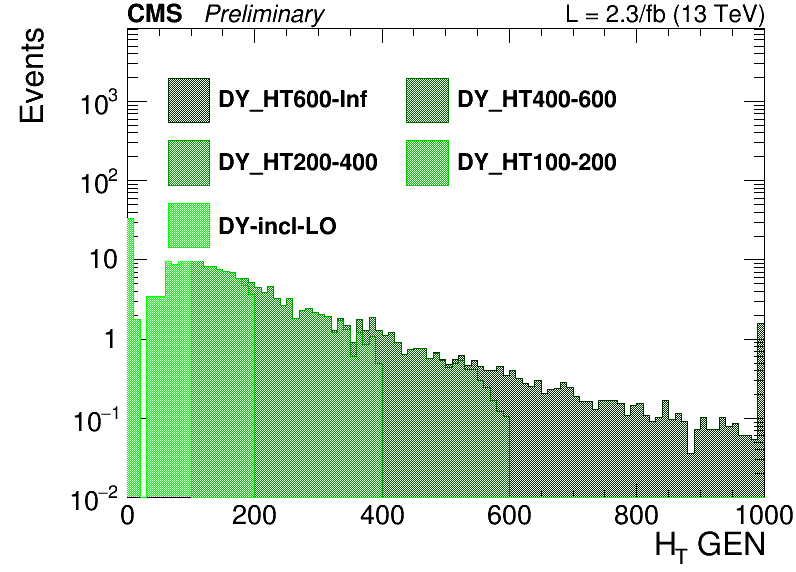
\includegraphics[width=0.5\textwidth]{images/13TeV/log_c_incl_HTGen.png}
\caption{
    Generator level $H_\mathrm{T}$ distribution for the merged DY sample.}
    \label{fig:DY_HT}
\end{figure}

In order to perform the resonance search in a large part of the mass spectrum, several signal samples for the gluon-gluon fusion and the vector boson fusion mechanisms have been generated corresponding to different Higgs boson masses in the range between 200\GeV and 1\TeV. The signal width for each mass point corresponds to the one expected for a SM Higgs boson at that mass. The samples are produced with a mass step of 50\GeV from 250 to 800\GeV and of 100\GeV from 800 to 1000\GeV. A finer stepping is used between 200 and 250\GeV. All the signal samples are generated with the \textsc{Powheg V2} generator, interfaced with the \textsc{JHUGen v6.2.8} generator, which handles the decay of the Higgs boson to $\mathrm{W^+ W^-}\to2\ell2\nu$.

The interference effects among gg$\to$X$\to$WW, gg$\to$WW and gg$\to$H$\to$WW are evaluated using the  \textsc{mcfm} and \textsc{JHUGen} generators, as implemented in the MELA framework~\cite{JHUGen}. Details about the interference effects are given in Sec.~\ref{chap6:AnalysisStrategy}.

\section{Analysis strategy}\label{chap6:AnalysisStrategy}

The analysis strategy for the first results on the high mass search in the $\mathrm{W^+W^-}\to2\ell2\nu$ decay channel closely follows the strategy presented in the 13\TeV SM Higgs search in the $\mathrm{H}\to\mathrm{W^+W^-}\to2\ell2\nu$ channel regarding the 0 and 1 jet categories. In addition a dedicated category to the VBF production mechanism is added, given that this production mode is particularly important in the high mass region. Indeed, assuming a SM Higgs boson, the ratio of cross sections $\sigma_\mathrm{VBF}/\sigma_\mathrm{ggH}$\footnote{The ggH notation is used for the gluon-gluon fusion production mode, even in the cases where a non-SM Higgs boson is created in the process.} increases with the Higgs boson mass, making the VBF production mechanism more and more important as the mass of the resonance approaches to high values.

This analysis is affected essentially by the same background processes as the SM Higgs boson search, with the difference that in this case the SM Higgs boson processes, including all production modes, are treated as backgrounds.

In addition to requiring the events to pass the single or double lepton triggers, exactly one electron and one muon are required to be reconstructed in the event with opposite charges and a 
minimum \pt of 20\GeV for both the muon and electron. Both leptons are
required to be well identified and isolated to reject fake leptons and leptons
coming from decays in flight. To suppress background processes with three or more leptons in the final state, such as diboson or triboson production, events with any additional identified and isolated 
lepton with $\pt>10$\GeV are rejected. To suppress the contribution of the SM production of the Higgs boson at 125\GeV, \mll is requested to be higher than 50\GeV. The other event requirements are identical to the 125\GeV Higgs boson search and are described in Sec.~\ref{chap5:eventSel}.

In addition to the 0 and 1 jet categories, a specific category sensitive to the VBF production mode is defined exploiting the characteristic signature of this process, where two energetic jets are emitted in the forward region of the detector and with large $\Delta\eta$ gap. Events belonging to the VBF-enriched category are selected by requiring at least two jets with $\pt>30$\GeV, an invariant mass $m_\mathrm{jj}>500$\GeV and a gap in pseudorapidity $\Delta\eta_\mathrm{jj}>3.5$.

In addition to the transverse mass variable \mt, which is used in the analysis selection to define the DY background control region, an additional variable is defined, that from now on will be labelled as ``improved transverse mass'' \mti. This variable is defined as the invariant mass of the four momentum resulting from the sum of the two leptons four momenta ($p_{\ell\ell},\vec{p}_{\ell\ell}$)
and four momentum $\mathbf{\MET} = (\MET, \ptmiss)$, i.e.:

\begin{equation} 
\mti = \sqrt{(p_{\ell\ell}+\MET)^2-(\vec{p}_{\ell\ell}+\ptmiss)^2} \quad .
\end{equation}

This variable allows having a better sensitivity to different resonance mass hypothesis as shown in Fig.~\ref{fig:mti}, where the shape of the \mti variable is shown for different SM Higgs mass hypothesis and it is compared to the standard \mt variable. The usage of this variable also provide a good discriminating power between signal and background, which depends on the particular signal mass hypothesis.

\begin{figure}[htbp]
\centering
\subfigure{
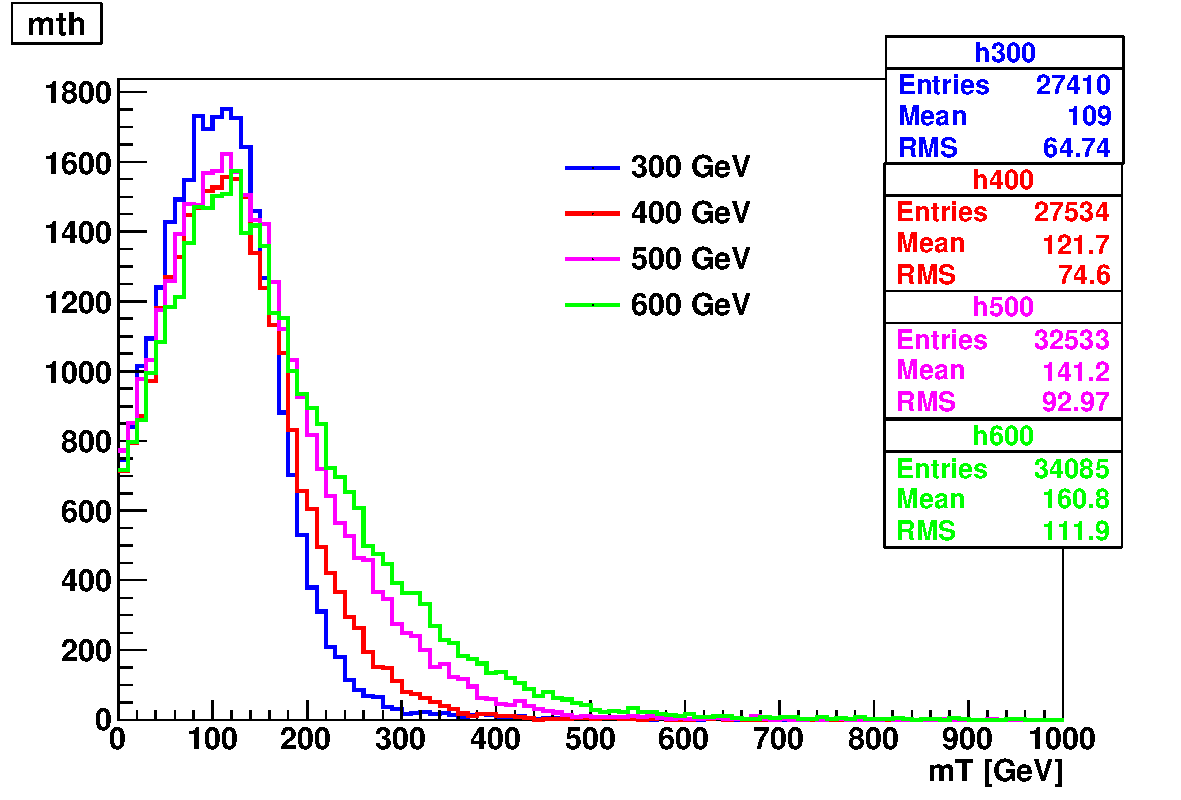
\includegraphics[width=0.45\textwidth]{images/13TeV/mT.pdf}
}
\subfigure{
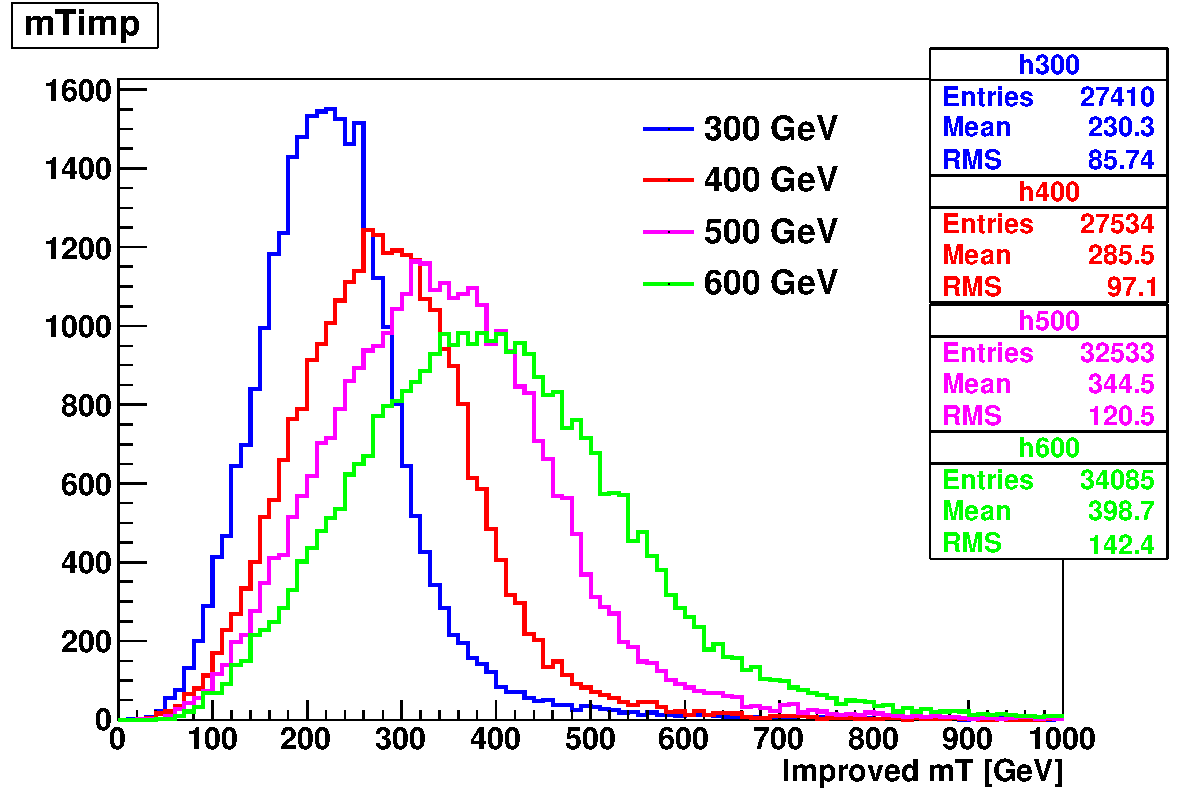
\includegraphics[width=0.45\textwidth]{images/13TeV/mTi.pdf}
}
\caption{
    Distribution of the \mt and \mti variables at generator level for different resonance mass hypothesis.}
    \label{fig:mti}
\end{figure}

The signal extraction is based on a binned maximum likelihood fit using the \mti distribution for signal and background contributions as templates. The \mti template is defined using the following bin boundaries:
\begin{itemize}
\item {\bf 0/1 jet: } [100,150,200,250,300,350,400,450,500,600,700,1000] ,
\item {\bf VBF: } [100,150,200,250,300,350,400,500,700,1000] ,
\end{itemize}
where the first number represents the lower edge of the first bin while the other numbers represent the upper edges. The last bin is an overflow bin.

In order to test different resonance decay widths hypotheses, the signal samples, which are generated with a decay width corresponding to the expected value for a SM Higgs boson at that mass ($\Gamma_\mathrm{SM}$), are reweighted to obtain the desired width value ($\Gamma'$). In particular the following values are used: $\Gamma' = \Gamma_\mathrm{SM}$, $\Gamma' = 0.49 \times \Gamma_\mathrm{SM}$, $\Gamma' = 0.25 \times \Gamma_\mathrm{SM}$ and $\Gamma' = 0.09 \times \Gamma_\mathrm{SM}$.





\section{Background estimation}\label{chap6:Backgrounds}

The background processes affecting the analysis phase space are the same as the ones contributing to the SM Higgs boson measurement described in Sec.~\ref{chap5:backgrounds}. The techniques used for the background estimation are the same as well.

The most relevant difference is the addition of the 2 jets category. The WW and top quark background normalizations are estimated in this category using data driven techniques, similarly to the other jet multiplicity categories.

Given the slightly different WW baseline selection with respect to the SM Higgs boson measurement, also the control regions for the top quark and \dytt backgrounds estimation are different, while the WW background normalization is estimated from data in the three signal regions separately, owing to the different \mti shapes for signal and background.

For the estimation of the top quark background, three control regions enriched in b-jets are defined by selecting events that pass the WW baseline selections and applying a b tagging requirement that depends on the jet category as follows:
\begin{itemize}
\item 0 jets category: at least one b-tagged jet with $20 < \pt < 30$\GeV is required;
\item 1 jet category: exactly one b-tagged jet with \pt above 30\GeV is required;
\item 2 jets category: at least one b-tagged jet with \pt above 30\GeV is required.
\end{itemize}
Distributions of the \mti variable in the 0 jets, 1 jet and 2 jets top quark enriched control regions after applying the data driven estimation are shown in Fig.~\ref{fig:TopCtrl}.

\begin{figure}[!htb]
\centering
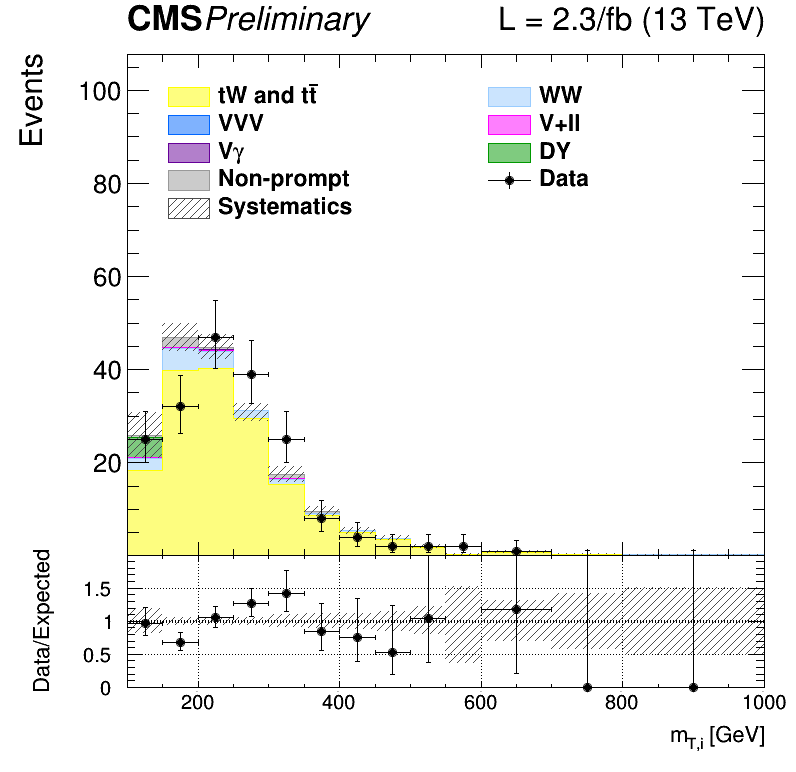
\includegraphics[width=0.45\textwidth]{images/13TeV/HighMass/cratio_hww2l2v_13TeV_top_of0j_mTi.png}
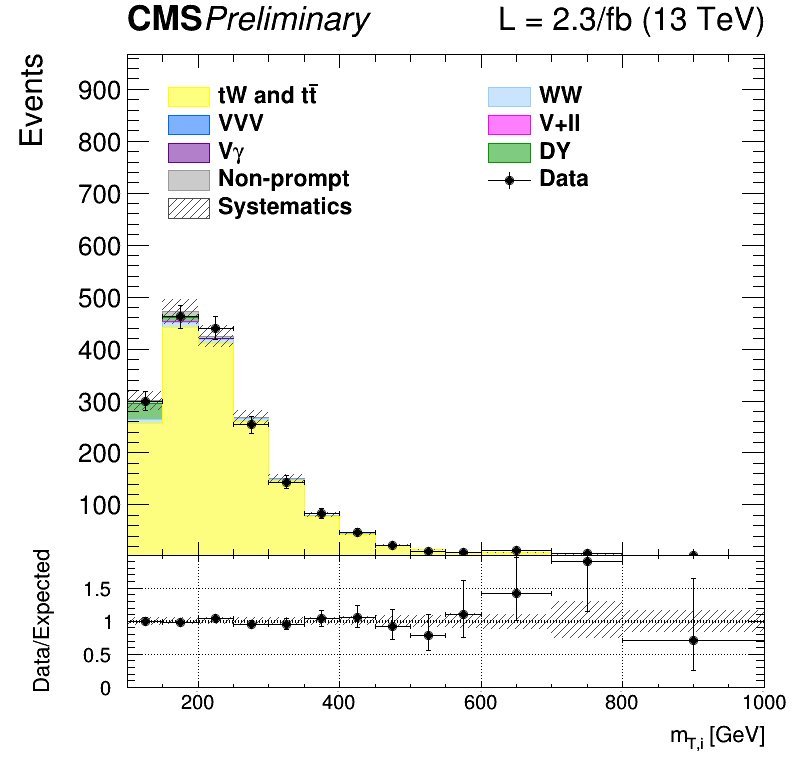
\includegraphics[width=0.45\textwidth]{images/13TeV/HighMass/cratio_hww2l2v_13TeV_top_of1j_mTi.png}
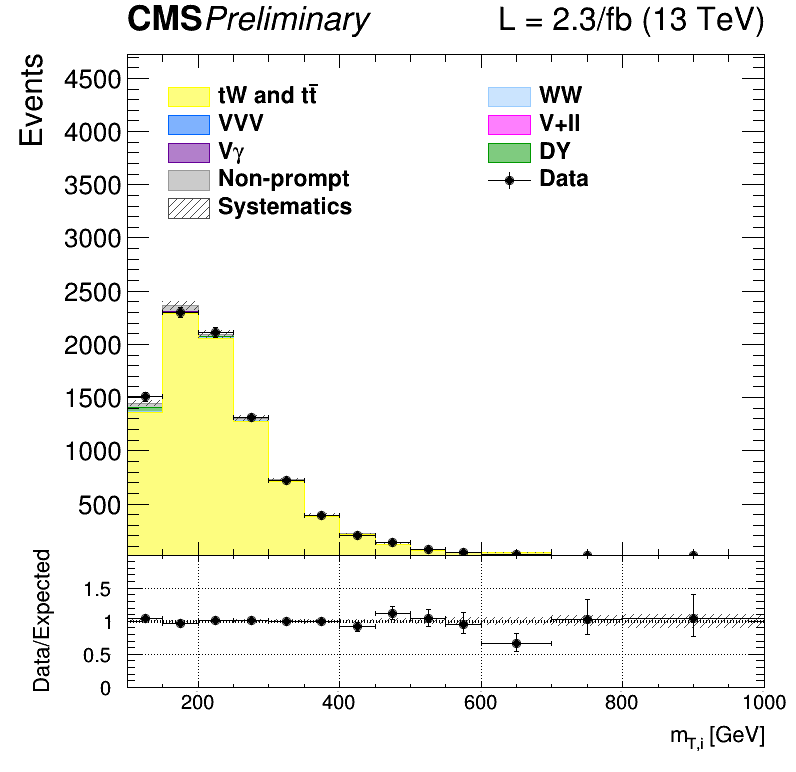
\includegraphics[width=0.45\textwidth]{images/13TeV/HighMass/cratio_hww2l2v_13TeV_top_of2j_mTi.png}
\caption{
Distributions of \mti for events with 0 jets (top left), 1 jet (top right)
and 2 jets (bottom) in top quark enriched control region.
Scale factors estimated from data are not applied. %Data points correspond to the 2015 data set.
}
\label{fig:TopCtrl}
\end{figure}

The jet induced background, here labelled as ``non-prompt'' background so as to highlight that these events do not contain prompt leptons, is estimated using the method described in Sec.~\ref{sec:wjetsbkg}. A cross-check is performed selecting events passing the WW baseline selection but containing an e$\mu$ pair with same charge. The \mti distributions for this phase space are illustrated in Fig.~\ref{fig:13TeV_hm_samesign} for the three jet categories, showing agreement between data and simulation within uncertainties.

\begin{figure}[htb]
\centering
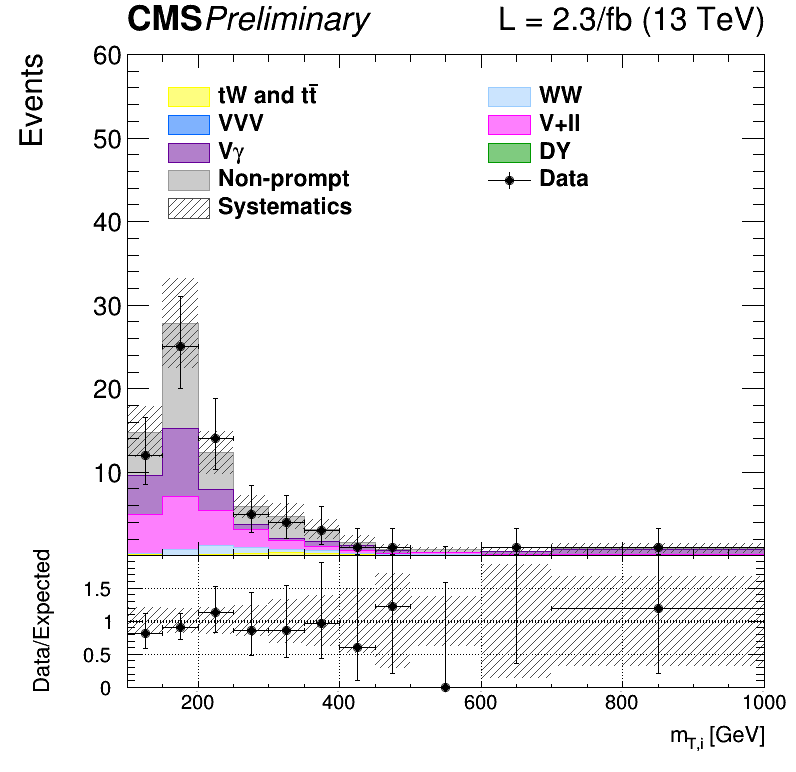
\includegraphics[width=0.45\textwidth]{images/13TeV/HighMass/cratio_hww2l2v_13TeV_ss_of0j_mTi_0j.png}
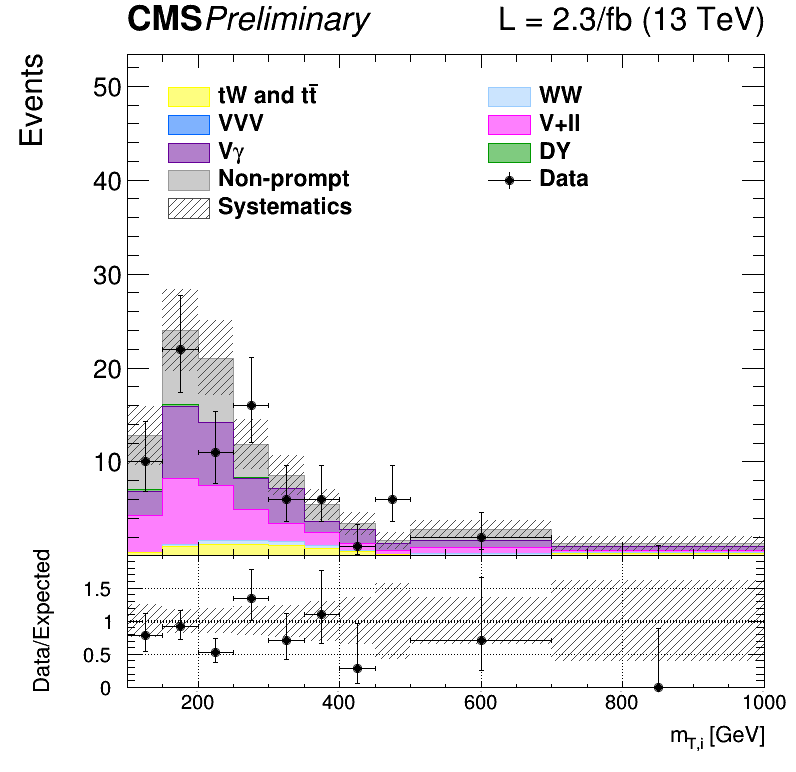
\includegraphics[width=0.45\textwidth]{images/13TeV/HighMass/cratio_hww2l2v_13TeV_ss_of1j_mTi_1j.png}
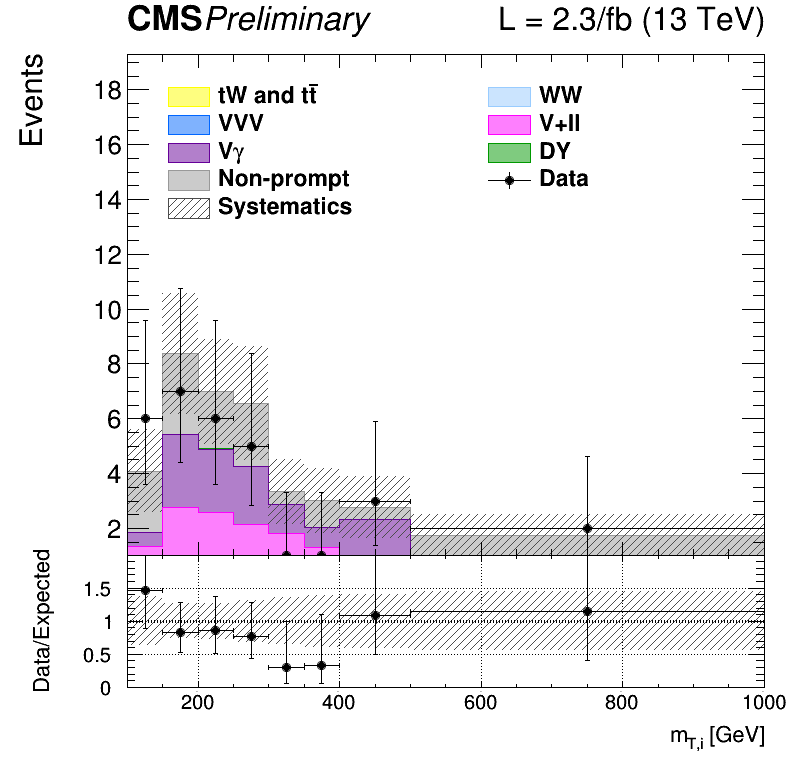
\includegraphics[width=0.45\textwidth]{images/13TeV/HighMass/cratio_hww2l2v_13TeV_ss_of2j_mTi_VBF.png}
\caption{
Distributions of \mti for events with 0 jets (top left), 1 jet (top right) and 2 jets (bottom) in the same-charge dilepton
control region. The last bin of the histograms includes overflows. %Data points correspond to the 2015 data set.
}
\label{fig:13TeV_hm_samesign}
\end{figure}

Due to the selections on the leptons \pt and on \mll in the WW baseline requirements, the contribution of the \dytt background is very small in the signal regions, especially in the VBF phase space. The normalization of this background is estimated from a control region in data, defined in the same way as explained in Sec.\ref{chap5:DYbackground}, for the 0 and 1 jets categories. In the VBF category the normalization of this background is taken from simulation.

Other minor background processes are estimated as described in Sec.~\ref{chap5:otherBackgrounds}.














\section{Systematic uncertainties}\label{chap6:Systematics}

The systematic uncertainties affecting this analysis are the same discussed in Sec.~\ref{chap5:systs}. The differences with respect to the Higgs boson cross section measurement presented in Chapter~\ref{chap5} are described below.

The PDF and $\alpha_s$ uncertainties on the signal cross sections are taken from the computations performed by the LHC cross section working group~\cite{YRtmp}, and are included for all the mass points. The value of these uncertainties depends on the resonance mass and vary from 3 to 5\% for ggH and from 2 to 3\% for VBF production modes. The PDFs and $\alpha_{s}$ uncertainties on the signal selection are evaluated for every resonance mass and are found to be less than 1\% for both ggH and VBF.

The theoretical uncertainties in the signal yields due to the jet categorization are evaluated for all the ggH signals following the prescription described in Refs.~\cite{Stewart:2011cf,Heinemeyer:2013tqa}.

An additional uncertainty on the modelling of the \ttbar background is derived from the observed discrepancy between data and \textsc{Powheg V2} plus \textsc{Pythia 8.1} simulation on the top quark \pt spectrum~\cite{Khachatryan:2015oqa}, which is particularly important in the tail of the \mti distribution. Another uncertainty affecting the \mti tail for the top quark background is the parton shower uncertainty. This is evaluated comparing the generator level \mti distributions corresponding to two different simulations of the \ttbar process: one obtained using \textsc{Pythia 8.1} for the showering and hadronization of the simulated events, and the other using \textsc{Herwig++}. The difference between the two is used to extract a shape uncertainty, which is less than 1\% for low \mti values and reaches about 6\% in the \mti tail.







\section{Signal extraction and limit setting}\label{chap6:SignalExtractionAndLimits}

The signal yield, including both ggH and VBF production modes, is extracted performing a combined fit of the three categories to the \mti simulation templates for backgrounds and signal, and is repeated for each resonance mass hypothesis. Moreover, fixed the mass of the resonance, the fit is performed again for the various hypotheses of the resonance decay width. A single signal strength $\mu$ is extracted from each fit, which multiplies both the ggH and VBF contributions. In other words the ratio of the two production mechanism is assumed to stay the same as the one predicted by the SM\footnote{This approximation limits the amount of models that can be tested with the provided results. A future development of this analysis, with larger integrated luminosity, might also include the cases for which different ggH and VBF relative contributions are expected.}.

The background yields expected from simulation corresponding to the three jet categories and after the analysis event selection are shown in Table~\ref{tab:bkg_yields}. The signal yields corresponding to a selection of mass points and assuming $\Gamma' = \Gamma_\mathrm{SM}$ are shown in Table~\ref{tab:sig_yields}.

\begin{table}[htb]
\begin{center}
\caption{Expected yields estimated from simulation (except for the non-prompt contribution which is estimated using data) for each background process in the three analysis categories, after the analysis event selection. The uncertainties are shown for the processes estimated from simulation.}\label{tab:bkg_yields}
\small{
\begin{tabular}{c c c c }
\toprule
             Background process           &         0 jets                                          &          1 jet                                         &        VBF                                           \\
\midrule
      $\mathrm{q\bar{q}'\to WW}$                &    501.93 $\pm$       0.00 (0\%)              &     198.72 $\pm$       0.00 (0\%)             &      4.54 $\pm$       0.00 (0\%)               \\
      $\mathrm{gg\to WW}$                &     37.28 $\pm$       5.77 (15\%)              &      19.63 $\pm$       3.04 (15\%)             &      1.05 $\pm$       0.16 (15\%)               \\
      Top quark                &    188.75 $\pm$       0.00 (0\%)              &     330.05 $\pm$       0.00 (0\%)             &     25.06 $\pm$       0.00 (0\%)               \\
      DY                &     33.24 $\pm$       0.00 (0\%)              &      12.99 $\pm$       0.00 (0\%)             &      0.28 $\pm$       0.00 (0\%)               \\
      Non-prompt                &     64.21 $\pm$      19.26 (30\%)              &      31.69 $\pm$       9.51 (30\%)             &      2.10 $\pm$       0.63 (30\%)               \\
      V$\gamma$                &     26.62 $\pm$       0.72  (3\%)              &      14.18 $\pm$       0.38  (3\%)             &      0.64 $\pm$       0.02 (3\%)               \\
     V$\gamma^*$                &      4.44 $\pm$       1.12 (25\%)              &       3.39 $\pm$       0.85 (25\%)             &      0.14 $\pm$       0.04 (25\%)               \\
     VZ                &     13.51 $\pm$       0.76  (6\%)              &      11.67 $\pm$       0.66 (6\%)             &      0.28 $\pm$       0.02 (6\%)               \\
     VVV                &      0.01 $\pm$       0.00 (3\%)              &       0.02 $\pm$       0.00 (3\%)             &      0.00 $\pm$       0.00 (3\%)               \\   
     
 SM $\mathrm{H\to WW}$           &      6.04 $\pm$       0.40  (7\%)              &       3.10 $\pm$       0.11 (5\%)             &      0.34 $\pm$       0.02 (7\%)               \\
 
 SM $\mathrm{H\to\tau\tau}$                &      0.50 $\pm$       0.05 (9\%)              &       0.43 $\pm$       0.04 (9\%)             &      0.04 $\pm$       0.00 (9\%)               \\
      
\midrule
    Total background          &    876.5               &     625.9           &     34.5          \\
\bottomrule
\end{tabular}
}
\end{center}
\end{table}

\begin{table}[htb]
\begin{center}
\caption{Expected signal yields for the ggH and VBF production modes estimated from simulation after the analysis event selection. The yields are shown in the three jet categories and correspond to a selection of mass values in the hypothesis $\Gamma' = \Gamma_\mathrm{SM}$. The errors correspond to the theoretical uncertainties in the signal estimation.}\label{tab:sig_yields}
\small{\begin{tabular}{c c c c } 
\toprule
                 Mass [GeV]                 &          0 jets    &          1 jet              & VBF           \\ 
\midrule
\multicolumn{4}{c}{ggH signal yields} \\
\midrule
 200                        &      90.21 $\pm$       6.67 (7\%)             &      37.47 $\pm$       1.81 (5\%)     &       1.25 $\pm$       0.26 (21\%)      \\
 400                        &      66.35 $\pm$       4.90 (7\%)             &      32.65 $\pm$       1.57 (5\%)     &       2.04 $\pm$       0.42 (21\%)      \\
 600                        &      13.86 $\pm$       1.05 (8\%)             &       8.56 $\pm$       0.44 (5\%)     &       0.68 $\pm$       0.14 (21\%)      \\
 800                        &       3.20 $\pm$       0.25 (8\%)             &       2.32 $\pm$       0.13 (6\%)     &       0.22 $\pm$       0.05 (21\%)      \\
 1000                       &       0.88 $\pm$       0.07 (8\%)             &       0.70 $\pm$       0.04 (6\%)     &       0.07 $\pm$       0.02 (21\%)      \\
\midrule
\multicolumn{4}{c}{VBF signal yields} \\
\midrule
 200                        &       1.54 $\pm$       0.06 (4\%)             &       6.18 $\pm$       0.25 (4\%)     &       5.05 $\pm$       0.20 (4\%)      \\
 400                        &       0.91 $\pm$       0.04 (4\%)             &       3.42 $\pm$       0.14 (4\%)     &       3.19 $\pm$       0.13 (4\%)      \\
 600                        &       0.50 $\pm$       0.02 (4\%)             &       1.95 $\pm$       0.08 (4\%)     &       1.88 $\pm$       0.08 (4\%)      \\
 800                        &       0.33 $\pm$       0.01 (4\%)             &       1.21 $\pm$       0.05 (4\%)     &       1.16 $\pm$       0.05 (4\%)      \\
 1000                       &       0.22 $\pm$       0.01 (4\%)             &       0.79 $\pm$       0.03 (4\%)     &       0.69 $\pm$       0.03 (4\%)      \\
\bottomrule
\end{tabular}
}
\end{center}
\end{table}

The strategy for computing the exclusion limits is based on the modified frequentist approach, also referred to as $\mathrm{CL_s}$, as described in~\cite{CMS-NOTE-2011-005}. The first step is to construct the likelihood function $\mathcal{L}(\mu,\theta)$:
\begin{equation}
\mathcal{L}(data|\mu,\theta) = Poisson(data|\mu\cdot s(\theta) + b(\theta))\cdot p(\tilde{\theta}|\theta) \quad,
\end{equation}
where $data$ represents the experimental observation, $s$ and $b$ are the expected signal and background yields respectively and $\theta$ is the full set of true values for the nuisance parameters constrained by the prior distribution functions $p(\tilde{\theta}|\theta)$. The default values assigned to the nuisance parameters are labelled as $\tilde{\theta}$.

For a binned shape analysis, $Poisson(data|\mu\cdot s + b)$ is the product of the Poisson probabilities to observe $n_i$ events in bin i, i.e.:
\begin{equation}
\prod_i \frac{(\mu\cdot s_i + b_i)^{n_i}}{n_i !} e^{-\mu\cdot s_i - b_i} \quad.
\end{equation}
In order to test the compatibility of the data with the signal plus background (or the background only) hypothesis, the test statistic $\tilde{q}_\mu$ is constructed based on the profile likelihood ratio:
\begin{equation}
\tilde{q}_\mu = -2 \ln{\frac{\mathcal{L}(data|\mu,\hat{\theta}_\mu)}{\mathcal{L}(data|\hat{\mu},\hat{\theta})	}}  \quad \mathrm{with} \quad 0 \leq \hat{\mu} \leq \mu \quad ,
\end{equation}
where $\hat{\theta}_\mu$ refers to the conditional maximum likelihood estimators of $\theta$, given the signal strength $\mu$. The parameter estimators $\hat{\mu}$ and $\hat{\theta}$ correspond to the global maximum of the likelihood. The $0 \leq \hat{\mu}$ constraint is imposed to have a positive signal yield, e.g. background underfluctuations are forbidden, while $\hat{\mu} \leq \mu$ is imposed to have a one-sided confidence interval. The observed test statistic for the signal strength $\mu$ under test is referred to as $\tilde{q}_\mu^\mathrm{obs}$. The values of the nuisance parameters obtained maximizing the likelihood function are labelled as $\hat{\theta}_0^\mathrm{obs}$ and $\hat{\theta}_\mu^\mathrm{obs}$ for the background only and signal plus background hypotheses, respectively. The pdf of the test statistic in constructed by generating toy MC pseudo-data for both the background only and signal plus background hypotheses, i.e. $f(\tilde{q}_\mu|\mu,\hat{\theta}_\mu^\mathrm{obs})$ and $f(\tilde{q}_\mu|0,\hat{\theta}_0^\mathrm{obs})$. These distributions can be used to define two p-values corresponding to the two hypotheses, $p_\mu$ and $p_b$:
\begin{equation}
p_\mu = P(\tilde{q}_\mu \geq \tilde{q}_\mu^\mathrm{obs}|\mathrm{signal+background}) = \int_{\tilde{q}_\mu^\mathrm{obs}}^{\infty} f(\tilde{q}_\mu|\mu,\hat{\theta}_\mu^\mathrm{obs}) d\tilde{q}_\mu \quad ,
\end{equation}
\begin{equation}
1 - p_b = (\tilde{q}_\mu \geq \tilde{q}_\mu^\mathrm{obs}|\mathrm{background~only}) = \int_{\tilde{q}_0^\mathrm{obs}}^{\infty} f(\tilde{q}_\mu|0,\hat{\theta}_0^\mathrm{obs}) d\tilde{q}_\mu \quad .
\end{equation}
According to these definitions, $p_\mu$ and $p_b$ can be identified with $\mathrm{CL_{s+b}}$ and $1-\mathrm{CL_b}$.
The $\mathrm{CL_s}(\mu)$ is calculated using the following ratio:
\begin{equation}
\mathrm{CL_s}(\mu) = \frac{\mathrm{CL_{s+b}}}{\mathrm{CL_b}} = \frac{p_\mu}{1-p_b} \quad .
\end{equation}
If, for a given signal strength $\mu$, $\mathrm{CL_s} \leq \alpha$, then the hypothesis is excluded with a $(1-\alpha)$ confidence level (CL). For instance, if one wants to quote the upper limit on $\mu$ with a 95\% CL, the signal strength has to be adjusted until $\mathrm{CL_s} = 0.05$.

The expected median upper limit, as well as the $\pm 1\sigma$ (68\% CL) and $\pm 2\sigma$ (95\% CL) bands, are determined generating a large amount of pseudo-data in the background only hypothesis and calculating $\mathrm{CL_s}$ and the 95\% CL upper limit for each of them, as if they were real data. Then the cumulative distribution of the 95\% CL upper limits is built and the median expected value is identified as the value at which the cumulative distribution crosses the 50\% quantile. The $\pm 1\sigma$ ($\pm 2 \sigma$) band is defined by the values at which the cumulative distribution crosses the 16\% (2.5\%) and 84\% (97.5\%) quantiles.

In order to assess the sensitivity of the analysis, the expected upper exclusion limits at 95\% CL on the signal strength are shown in Fig.~\ref{fig:13TeVexplim} for the three jet categories separately. For a given mass of the resonance, the limits are derived assuming a signal decay width $\Gamma' = \Gamma_\mathrm{SM}$ and a cross section equal to the one expected for a SM Higgs boson at that mass. The other decay width hypotheses have been tested as well, showing a very similar expected exclusion limit, suggesting that this analysis is not strongly sensitive to variations of the resonance decay width. In fact, the width of the \mti distribution is driven by the experimental resolution and the choice of different decay widths has only a mild effect on this variable.

The 0 jets category is the most sensitive especially in the low mass region, while for very large masses of the resonance the 1 jet and VBF categories start being important. This is explained mainly by the fact that the VBF contribution increases, with respect to ggH, as the mass increases. The expected exclusion limit on the signal strength after the combination of the three categories is shown in Fig.~\ref{fig:13TeVcombexplim}. Comparing the limits in the single categories with the combination of the three, it is evident how higher jet multiplicity categories help in improving the results for large values of $M_\mathrm{X}$. For the analysed luminosity the expected exclusion mass range for the production of a resonance with the SM Higgs boson cross section extends roughly from 350 to 450\GeV.

\begin{figure}[!htb]
\centering
\subfigure[0 jets]{
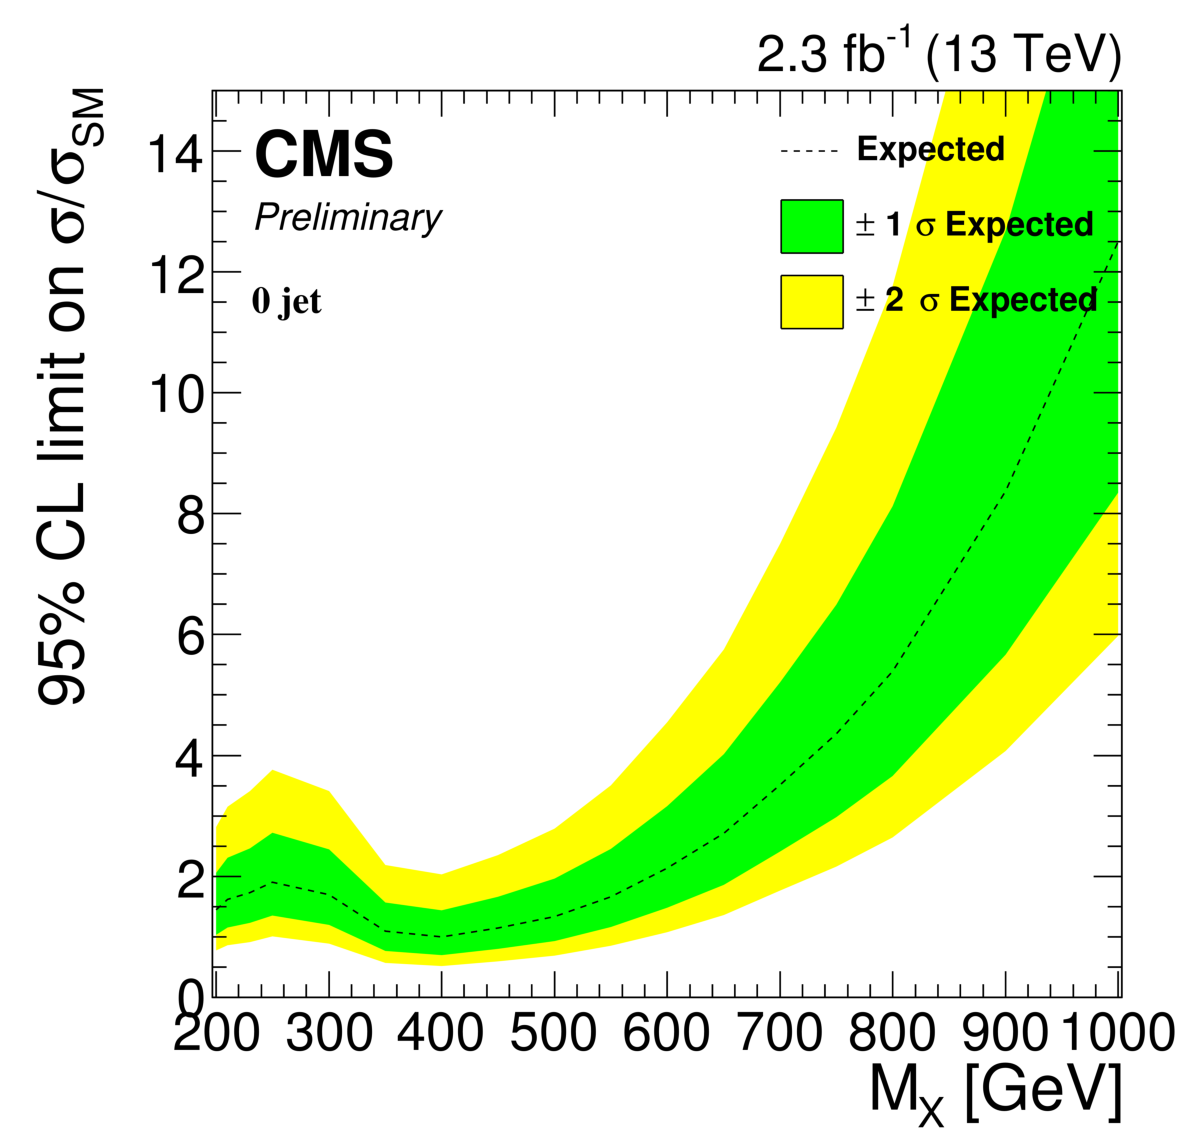
\includegraphics[width=0.31\textwidth]{images/13TeV/HighMass/exp_limit_0jet_mu.pdf}
}
\subfigure[1 jet]{
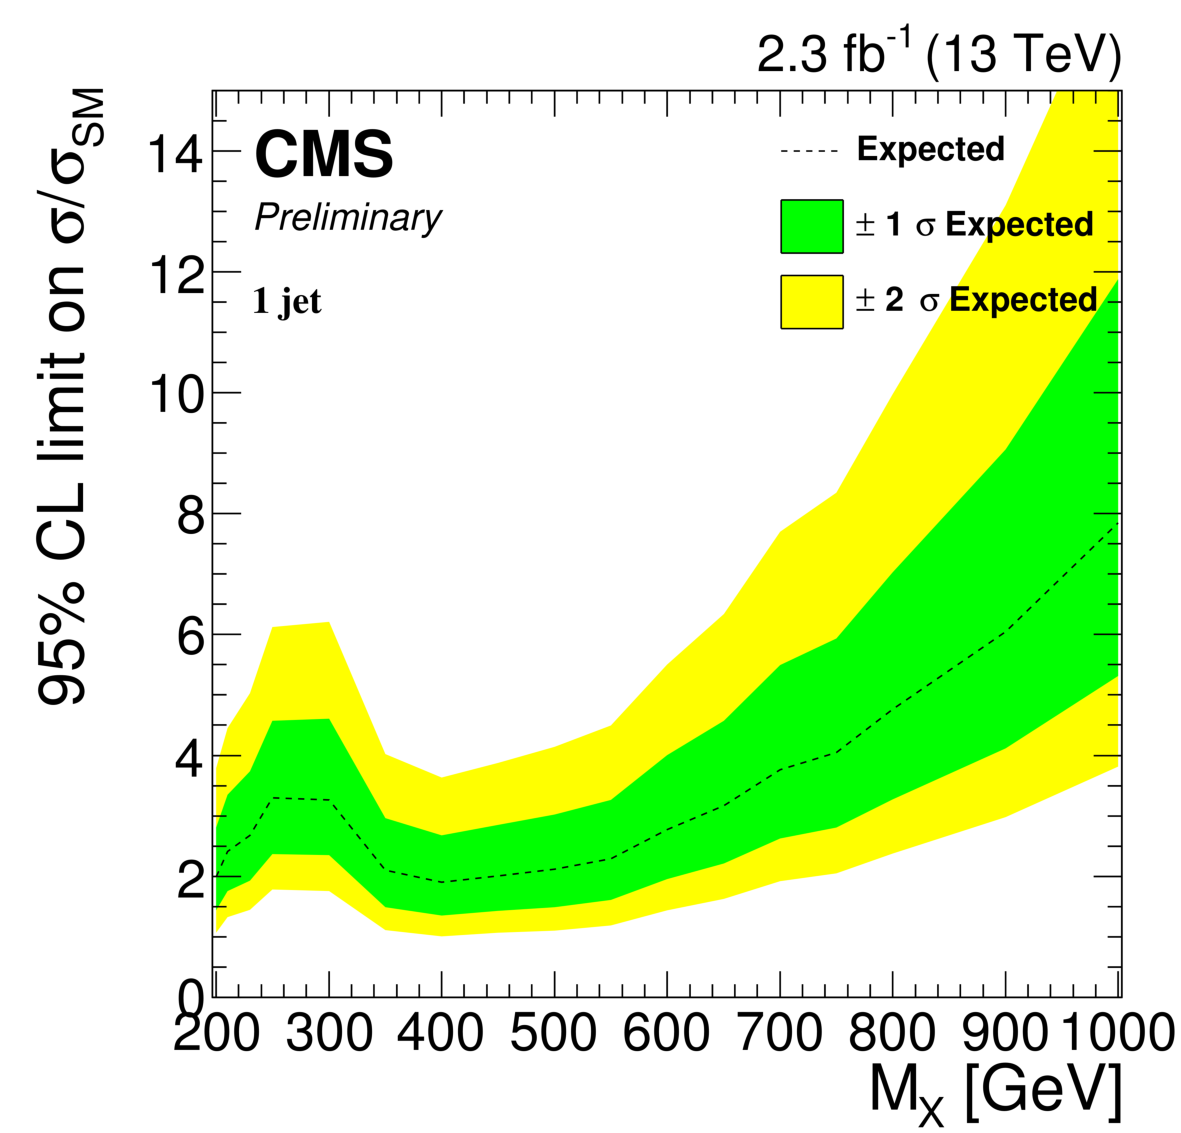
\includegraphics[width=0.31\textwidth]{images/13TeV/HighMass/exp_limit_1jet_mu.pdf}
}
\subfigure[VBF]{
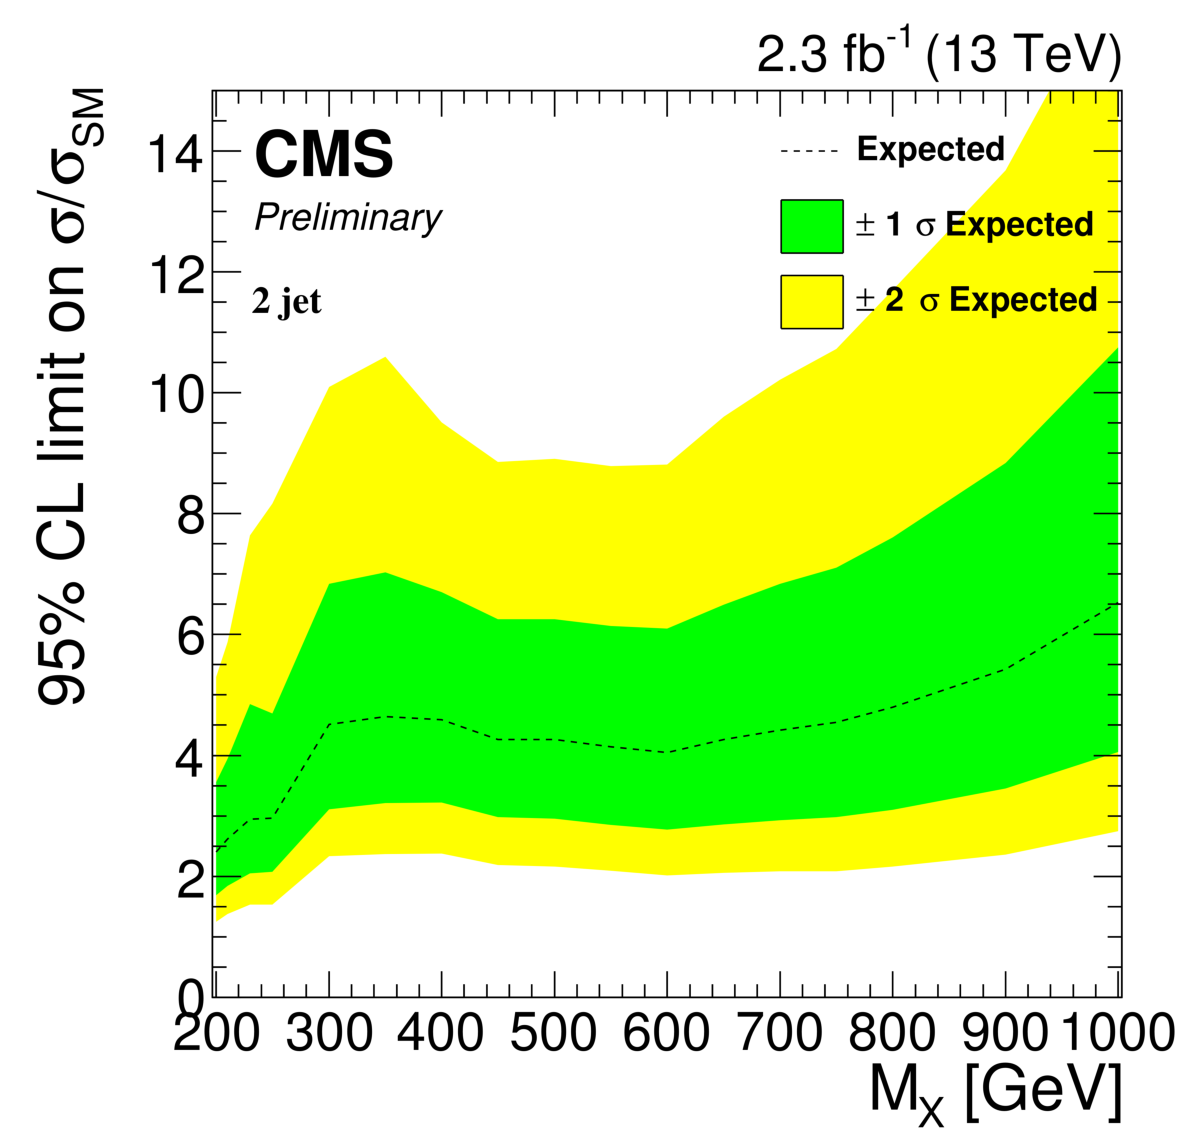
\includegraphics[width=0.31\textwidth]{images/13TeV/HighMass/exp_limit_2jet_mu.pdf}
}
\caption{Expected exclusion upper limits at 95\% CL on the signal strength in the three categories, as a function of the resonance mass. The dashed line corresponds to the median upper limit, while the green and yellow regions represent the $\pm 1\sigma$ and $\pm 2 \sigma$ uncertainty bands, respectively. Limits are derived assuming the SM Higgs boson cross section and decay width for each mass point.}\label{fig:13TeVexplim}
\end{figure}

\begin{figure}[!htb]
\centering
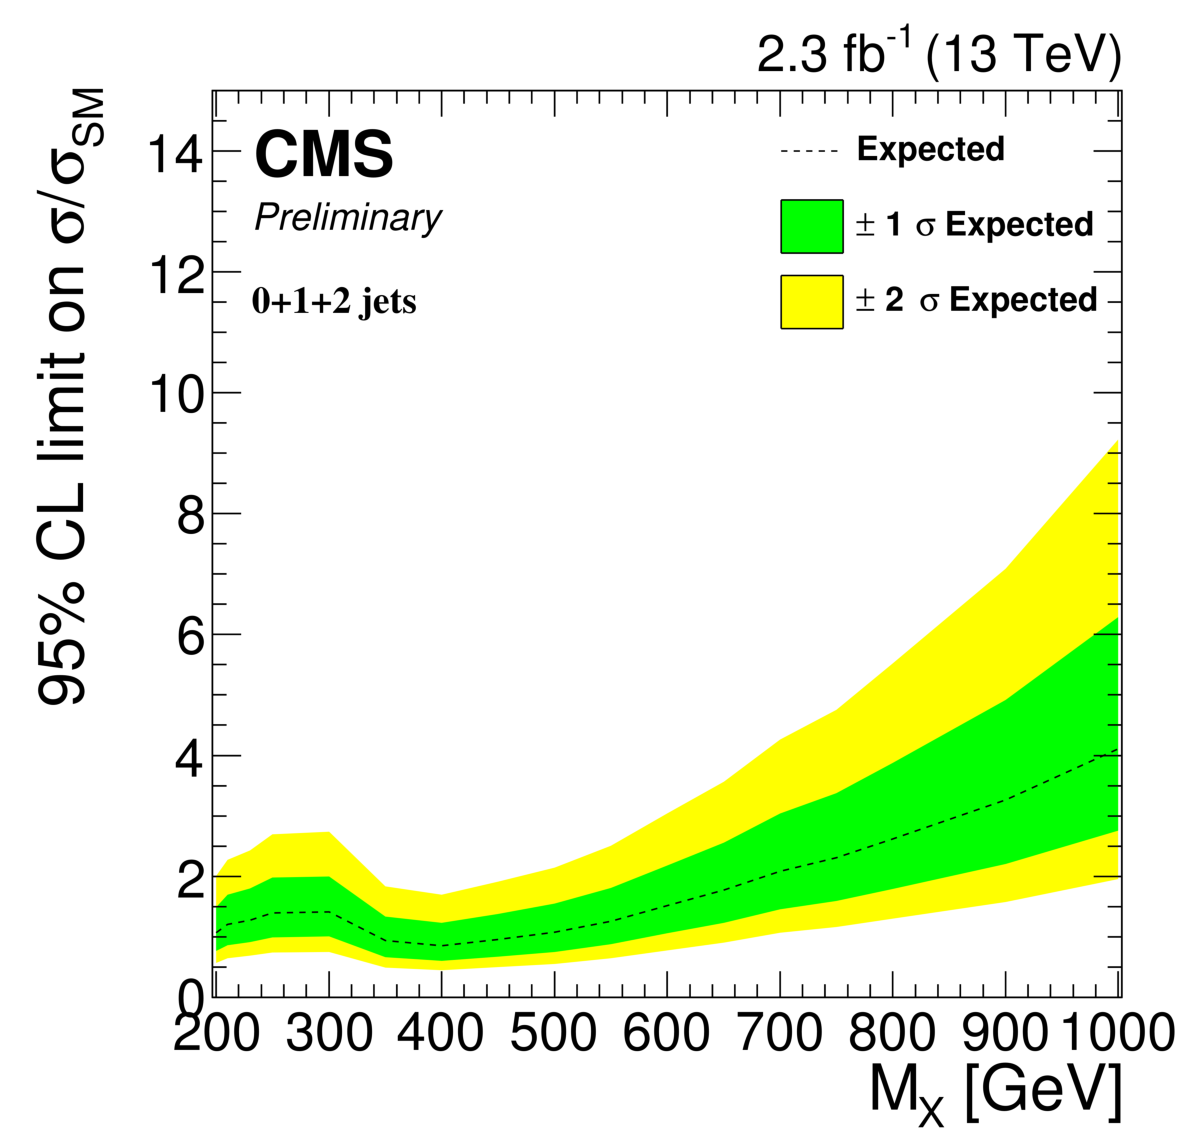
\includegraphics[width=0.5\textwidth]{images/13TeV/HighMass/exp_limit_012jet_mu.pdf}
\caption{Expected exclusion upper limit at 95\% CL on the signal strength for the combination of the three categories, as a function of the resonance mass. The dashed line corresponds to the median upper limit, while the green and yellow regions represent the $\pm 1\sigma$ and $\pm 2 \sigma$ uncertainty bands, respectively. The limit is derived assuming the SM Higgs boson cross section and decay width for each mass point.}\label{fig:13TeVcombexplim}
\end{figure}




\section{Results}\label{chap6:Results}

The \mti{} distributions for the signal region after the full analysis selection
are shown in Fig.~\ref{fig:13TeVmTishapes} for the three jet categories.
 Two different signal hypotheses corresponding to $M_\mathrm{X} = 400$\GeV and
 $M_\mathrm{X} = 800$\GeV are shown superimposed on the background for comparison.

\begin{figure}[!htb]
\centering
\subfigure[0 jets]{
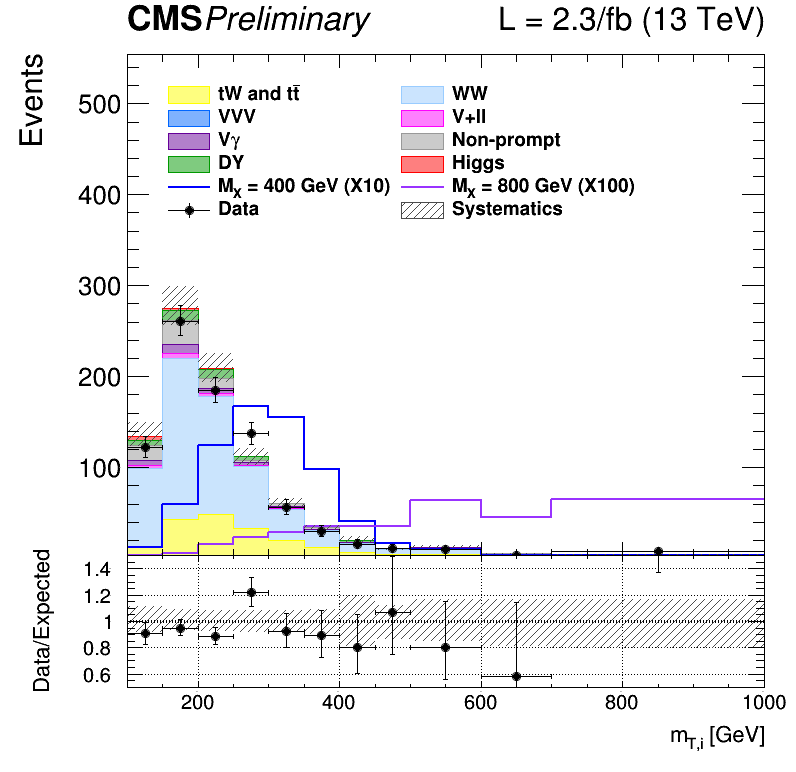
\includegraphics[width=0.45\textwidth]{images/13TeV/HighMass/cratio_hwwhm_13TeV_of_0j_mTi.png}
}
\subfigure[1 jet]{
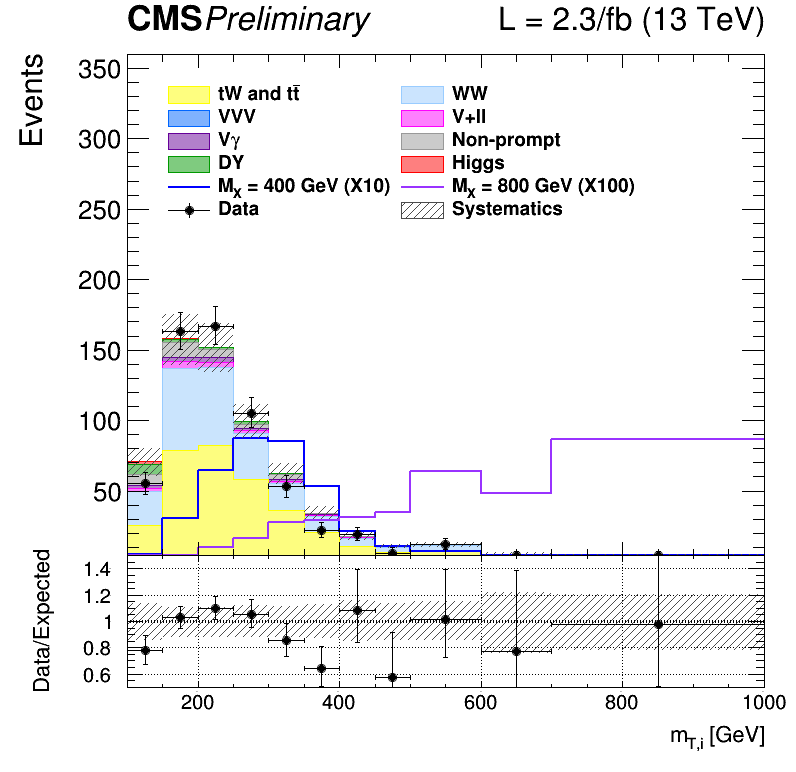
\includegraphics[width=0.45\textwidth]{images/13TeV/HighMass/cratio_hwwhm_13TeV_of_1j_mTi.png}
}
\\
\subfigure[VBF]{
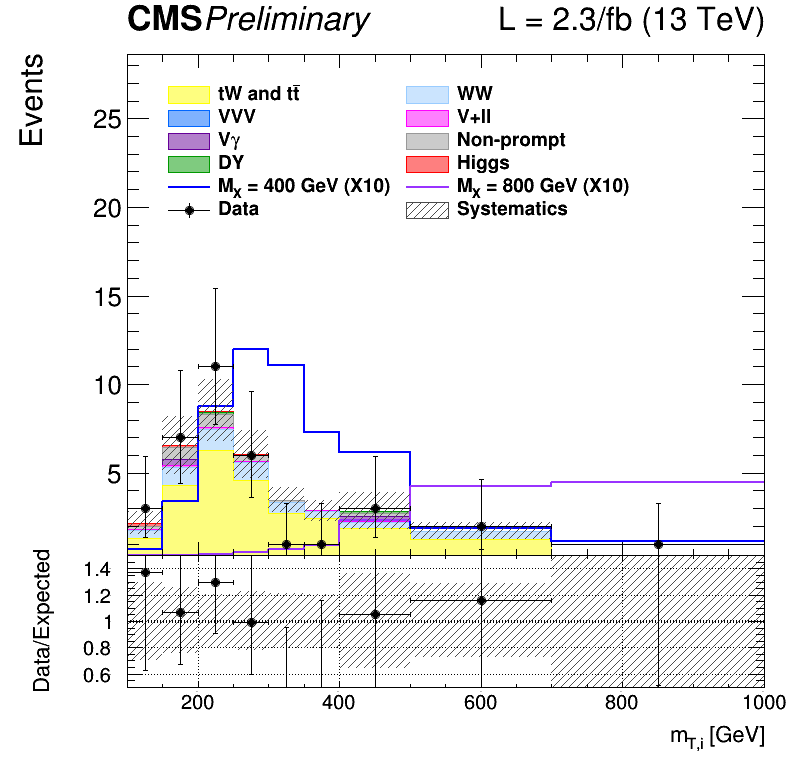
\includegraphics[width=0.45\textwidth]{images/13TeV/HighMass/cratio_hwwhm_13TeV_of_VBF_mTi_VBF.png}
}
\caption{
    Distributions of \mti{} in the signal region for the 0 jets, 1 jet and VBF categories. Background normalization corresponds to the pre-fit value. Signal contributions for two mass hypotheses, $M_\mathrm{X} = 400$\GeV and $M_\mathrm{X} = 800$\GeV, are shown superimposed on the background and scaled to facilitate the comparison.}
    \label{fig:13TeVmTishapes}
\end{figure}

For every mass point from 200\GeV up to 1\TeV the observed p-value and the 95\% CL upper exclusion limit are calculated for four hypotheses of the signal decay width. The observed p-value as a function of the resonance mass for the combination of the three jet categories is shown in Table~\ref{tab:significance}.

\begin{table}[htb]
\small{
\begin{center}
\caption{Observed p-value and corresponding significance (set to 0 in case of underfluctuations of the observed number of events) for the combination of the three jet categories for different resonance masses. Different values of the signal width are shown.\label{tab:significance}}
\begin{tabular}{lcccccc}
\toprule
\multirow{2}{*}{Mass [GeV]}            & $\Gamma = 0.09 \times \Gamma_{SM}$ & $\Gamma = 0.25 \times \Gamma_{SM}$ & $\Gamma = 0.49 \times \Gamma_{SM}$ & $\Gamma = \Gamma_{SM}$\\
                                          & p-value (signif.)  & p-value (signif.)  & p-value (signif.)  & p-value (signif.) \\
\midrule
200 &  0.50 (0)   & 0.50 (0)    & 0.50 (0) & 0.56 (0)\\
210 &  0.58 (0)   & 0.45 (0.1) & 0.35 (0.4) & 0.24 (0.7)\\
230 &  0.21 (0.8) & 0.22 (0.8) & 0.23 (0.7) & 0.26 (0.6)\\
250 &  0.29 (0.5) & 0.20 (0.8)  & 0.15 (1.0) & 0.12 (1.2)\\
300 &  0.014 (2.2)& 0.015 (2.2)& 0.016 (2.1) & 0.018 (2.1)\\
350 &  0.16 (1.0) & 0.17 (1.0) & 0.18 (0.9) & 0.23 (0.7)\\
400 &  0.50 (0)   & 0.49 (0)   & 0.49 (0) & 0.57 (0)\\
450 &  0.51 (0)   & 0.50 (0)   & 0.50 (0) & 0.52 (0)\\
500 &  0.50 (0)   & 0.51 (0)   & 0.50 (0) & 0.52 (0)\\
550 &  0.50 (0)   & 0.51 (0)   & 0.51 (0) & 0.51 (0)\\
600 &  0.50 (0)   & 0.50 (0)   & 0.51 (0) & 0.51 (0)\\
650 &  0.50 (0)   & 0.50 (0)   & 0.54 (0) & 0.50 (0)\\
700 &  0.50 (0)   & 0.50 (0)   & 0.50 (0) & 0.50 (0)\\
750 &  0.50 (0)   & 0.54 (0)   & 0.50 (0) & 0.40 (0.3)\\
800 &  0.50 (0)   & 0.55 (0)   & 0.39 (0.3) & 0.29 (0.6)\\
900 &  0.29 (0.6) & 0.27 (0.6) & 0.24 (0.7) & 0.22 (0.8)\\
1000 & 0.18 (0.9) & 0.18 (0.9) & 0.18 (0.9) & 0.18 (0.9)\\
\bottomrule
\end{tabular}
\end{center}
}
\end{table}

In order to be independent on the particular model assumed for the signal cross section, the results are interpreted as exclusion limits on $\sigma \times \mathcal{B}$, where $\sigma$ stands for the sum of the ggH and VBF cross sections, and $\mathcal{B}$ represents the $\mathrm{X\to WW \to2\ell2\nu}$ branching ratio including all lepton flavours. The expected and observed upper exclusion limits on $\sigma \times \mathcal{B}$ for $\Gamma' = \Gamma_\mathrm{SM}$ are shown in Fig.~\ref{fig:13TeVobslim}.

\begin{figure}[htb]
\centering
\subfigure[0 jets]{
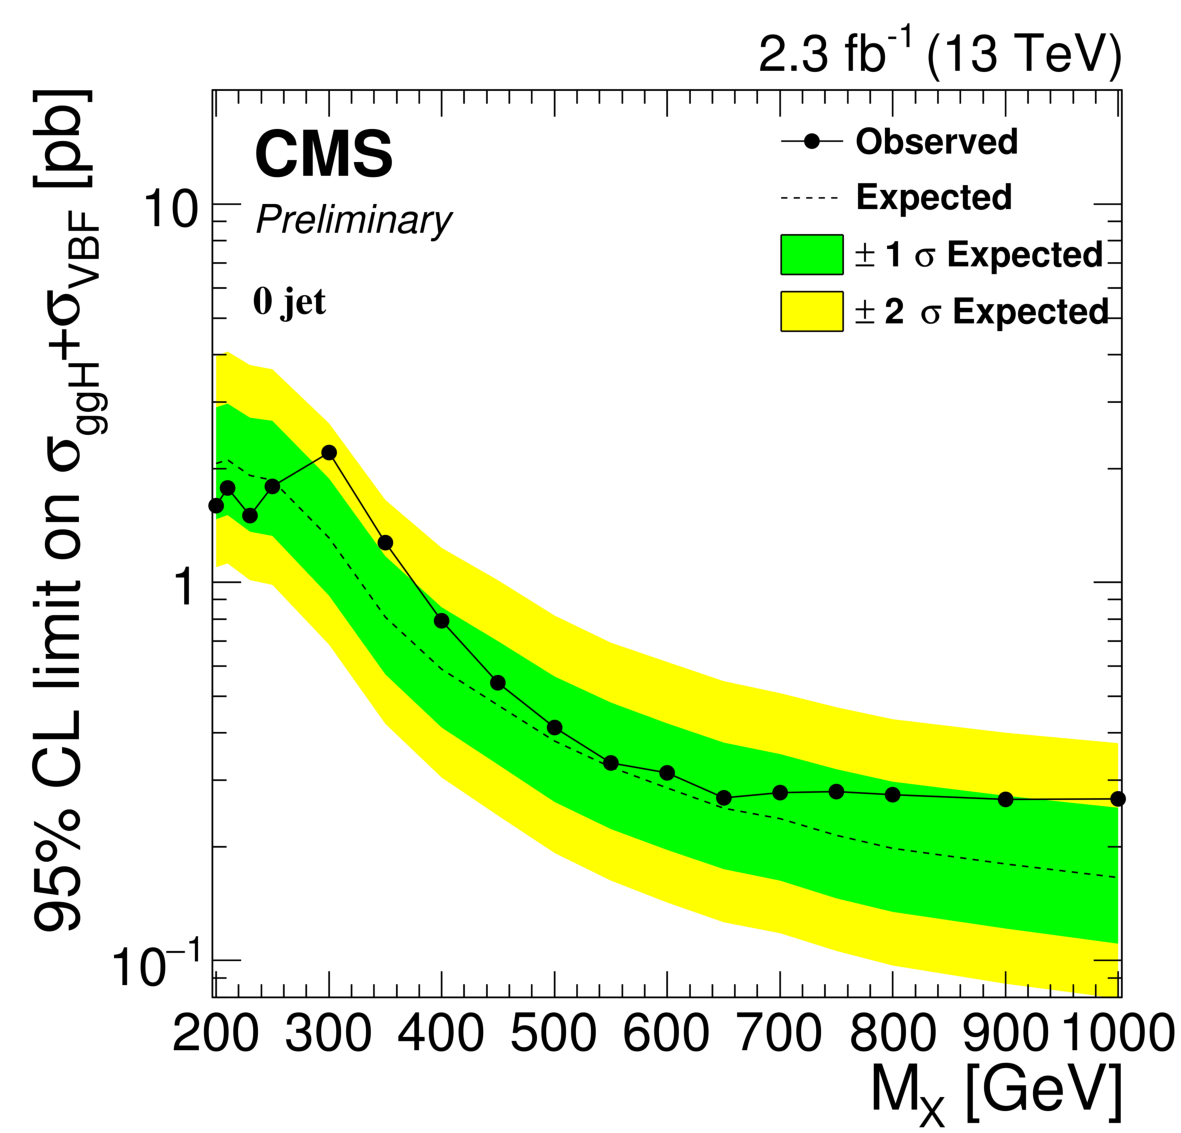
\includegraphics[width=0.45\textwidth]{images/13TeV/HighMass/obs_limit_0jet_xsec.pdf}
}
\subfigure[1 jet]{
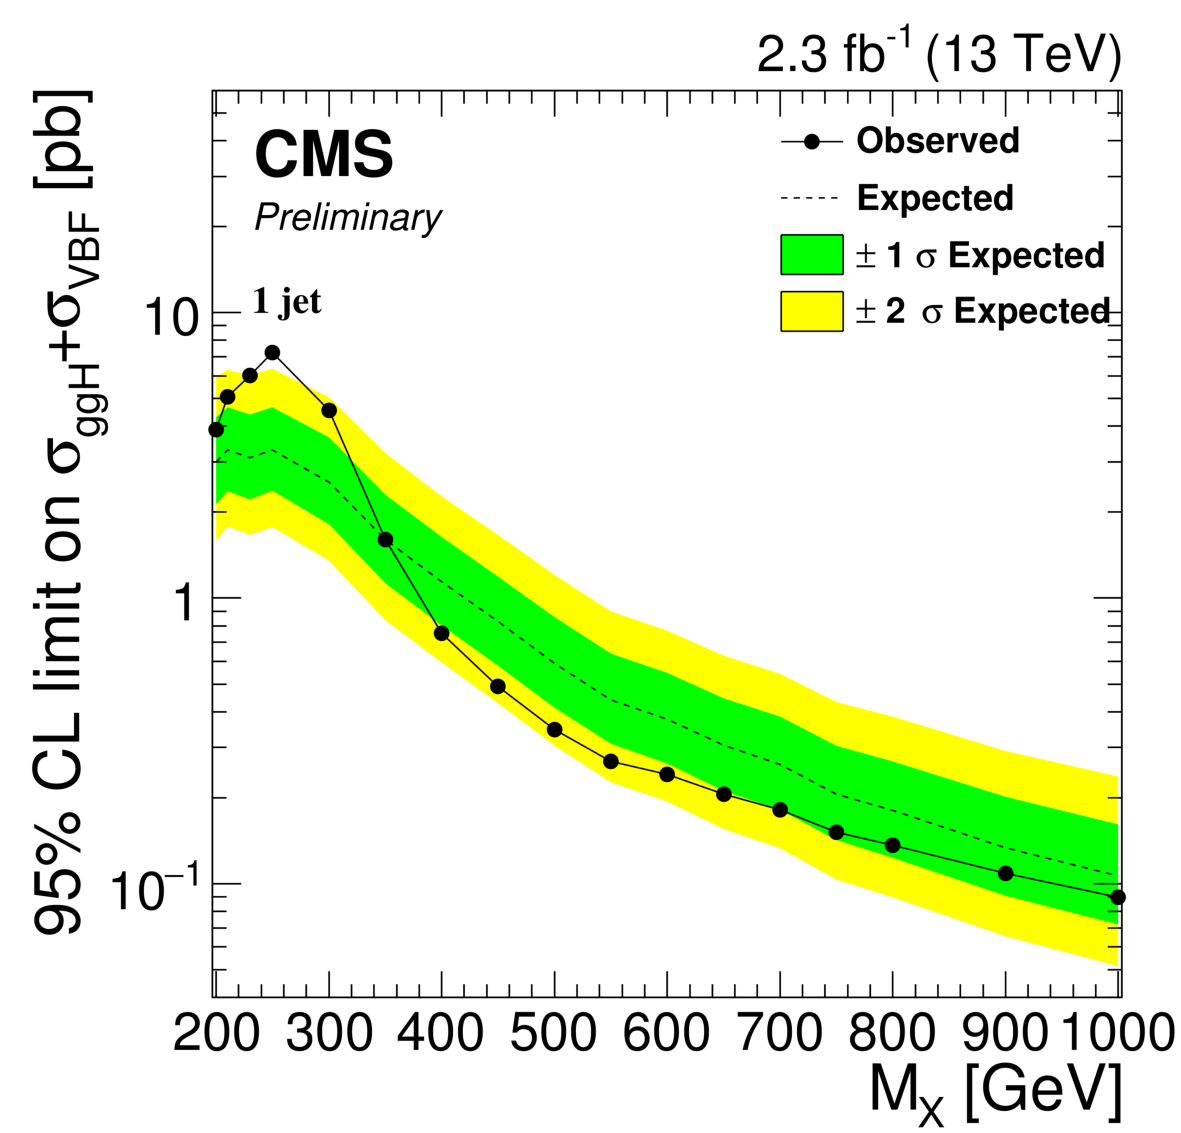
\includegraphics[width=0.45\textwidth]{images/13TeV/HighMass/obs_limit_1jet_xsec.pdf}
}\\
\subfigure[VBF]{
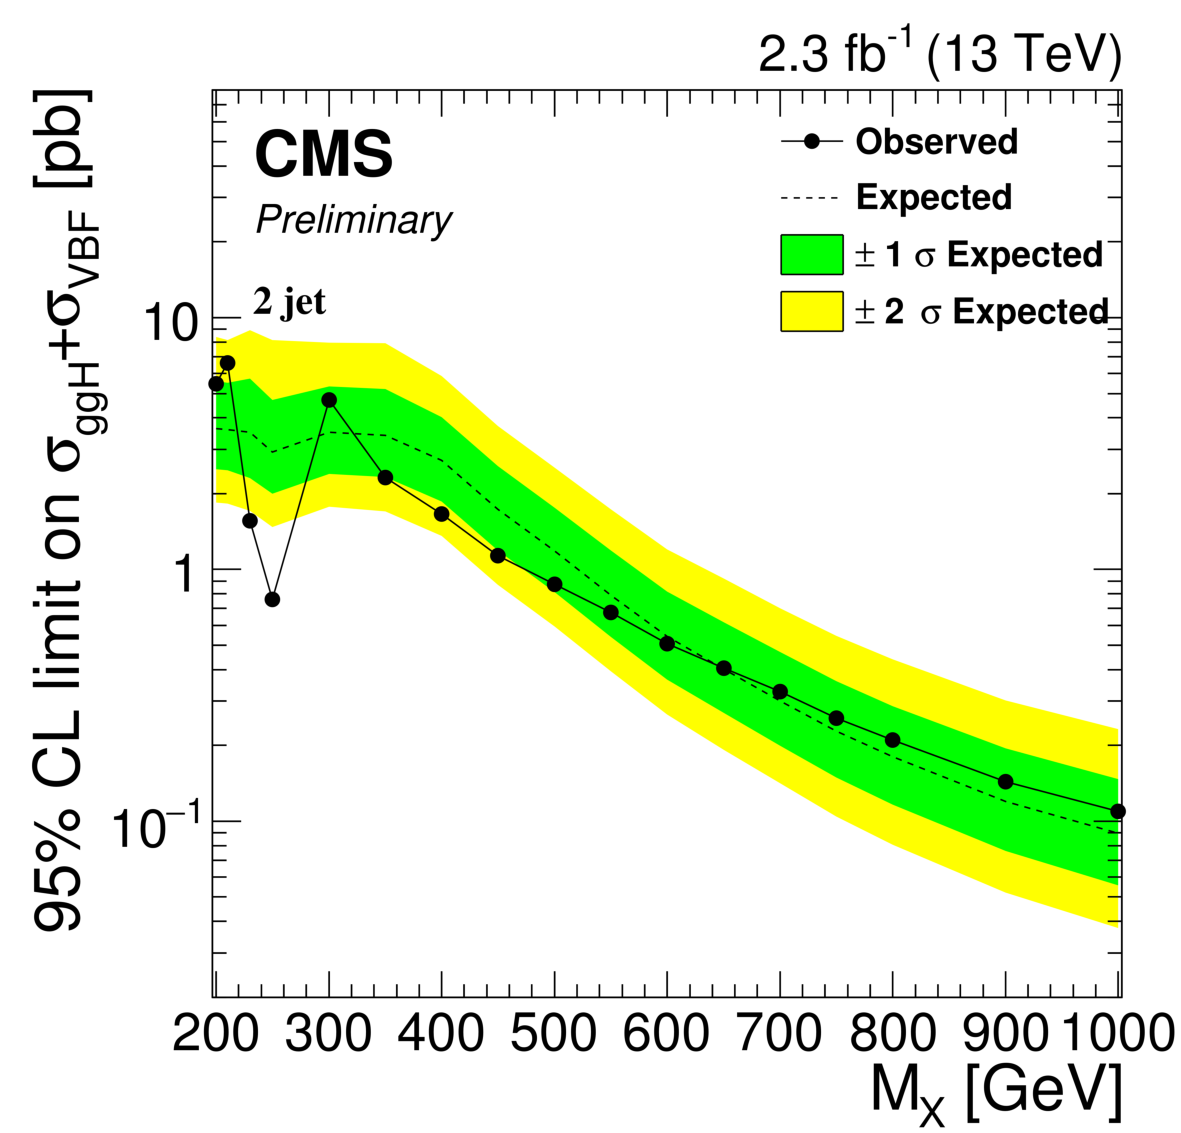
\includegraphics[width=0.45\textwidth]{images/13TeV/HighMass/obs_limit_2jet_xsec.pdf}
}
\caption{Expected and observed exclusion upper limits at 95\% CL on $\sigma \times \mathcal{B}$ in the three categories, as a function of the resonance mass. The dashed line corresponds to the median upper limit, while the green and yellow regions represent the $\pm 1\sigma$ and $\pm 2 \sigma$ uncertainty bands, respectively. The dotted line represents the observed limit. Limits are derived assuming $\Gamma' = \Gamma_\mathrm{SM}$ for each mass point.}\label{fig:13TeVobslim}
\end{figure}

A mild excess is observed in the 0 jets category and, more evident, in the 1 jet category around 250--300\GeV. A deficit is instead observed in the VBF category around 250\GeV, which is mainly due to an underfluctuation of the background. This effect can be understood looking at the distribution in the VBF category in Fig.~\ref{fig:13TeVmTishapes}, where two adjacent data points, corresponding to the fifth and sixth bins of the \mti distribution, clearly underfluctuate with respect to the background prediction, causing the dip in the observed limit.

The exclusion limit resulting from the combination of the three categories is shown in Fig.~\ref{fig:13TeVcombobslim}, for the four $\Gamma'$ hypotheses discussed before. From the combined exclusion limits no significant evidence of a deviation from the background only hypothesis is observed. In the case the new resonance has the same decay width as the SM Higgs boson, i.e. $\Gamma'=\Gamma_\mathrm{SM}$, the expected cross section times branching ratio is also displayed, excluding this hypothesis in the mass range from 370 to 550\GeV.
%The presence of a scalar resonance with $\sigma\times\mathcal{B}$ higher than the values reported in Fig.~\ref{fig:13TeVcombobslim} is thus excluded with a 95\% CL for masses ranging from 200\GeV up to 1\TeV. 

\begin{figure}[htb]
\centering
\subfigure{
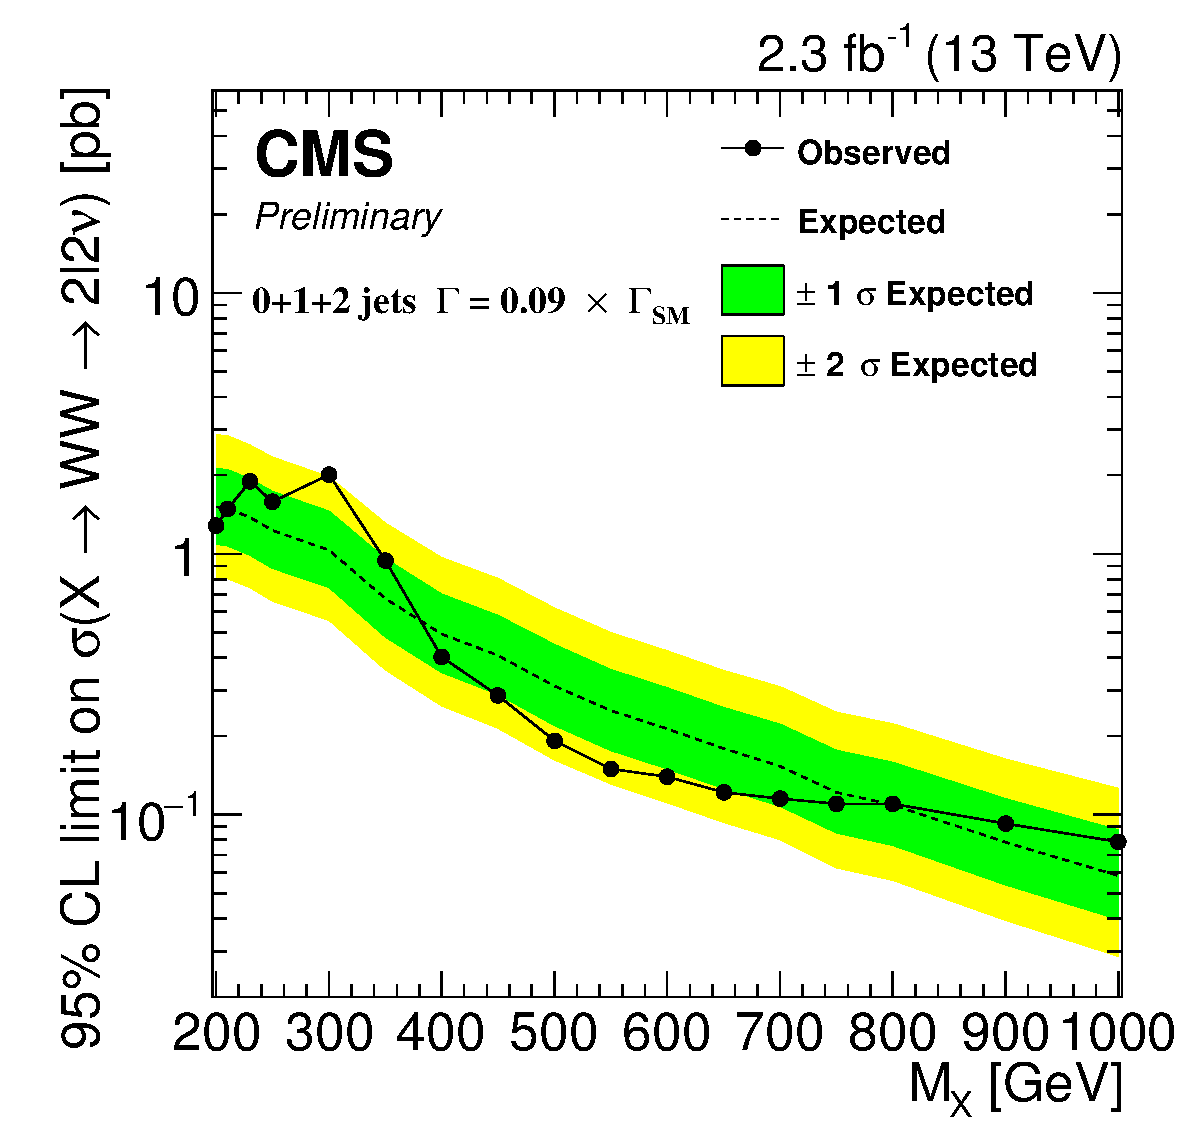
\includegraphics[width=0.45\textwidth]{images/13TeV/HighMass/limit_009GSM_PAS.pdf}
}
\subfigure{
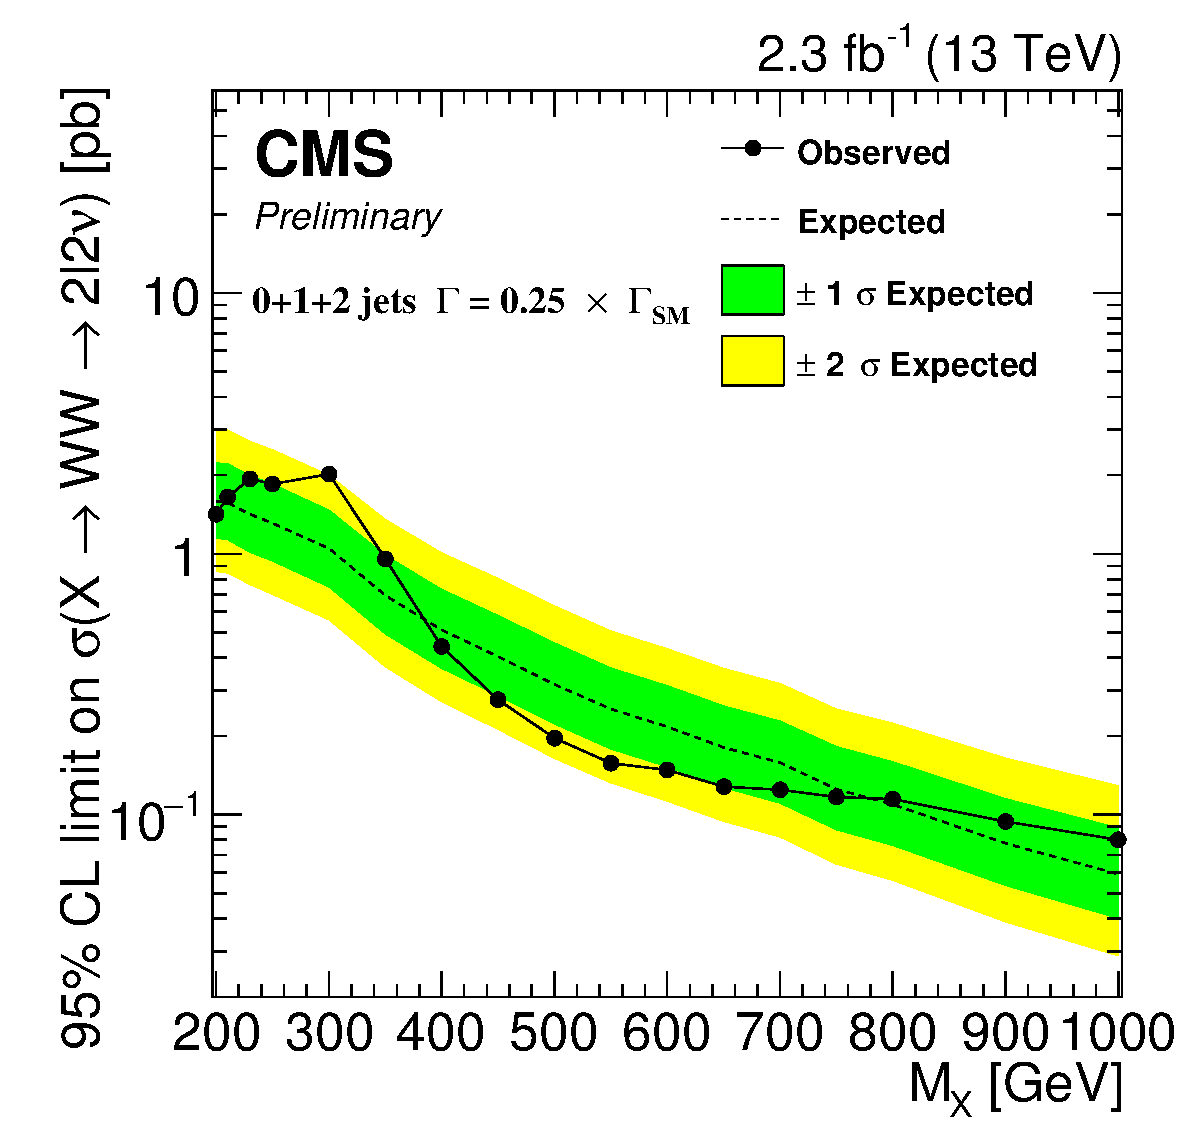
\includegraphics[width=0.45\textwidth]{images/13TeV/HighMass/limit_025GSM_PAS.pdf}
}
\\
\subfigure{
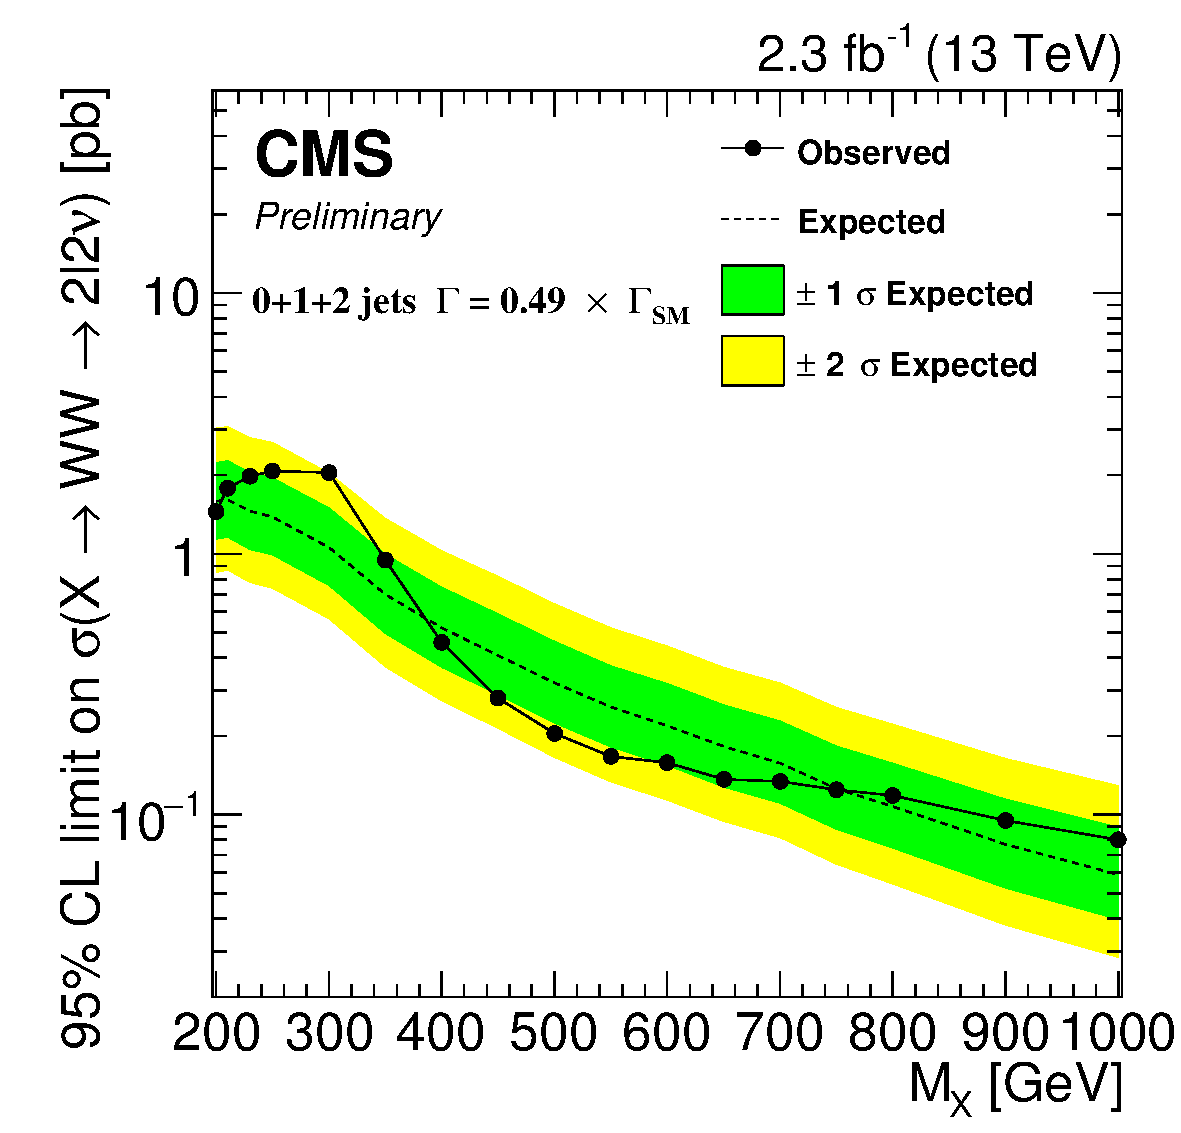
\includegraphics[width=0.45\textwidth]{images/13TeV/HighMass/limit_049GSM_PAS.pdf}
}
\subfigure{
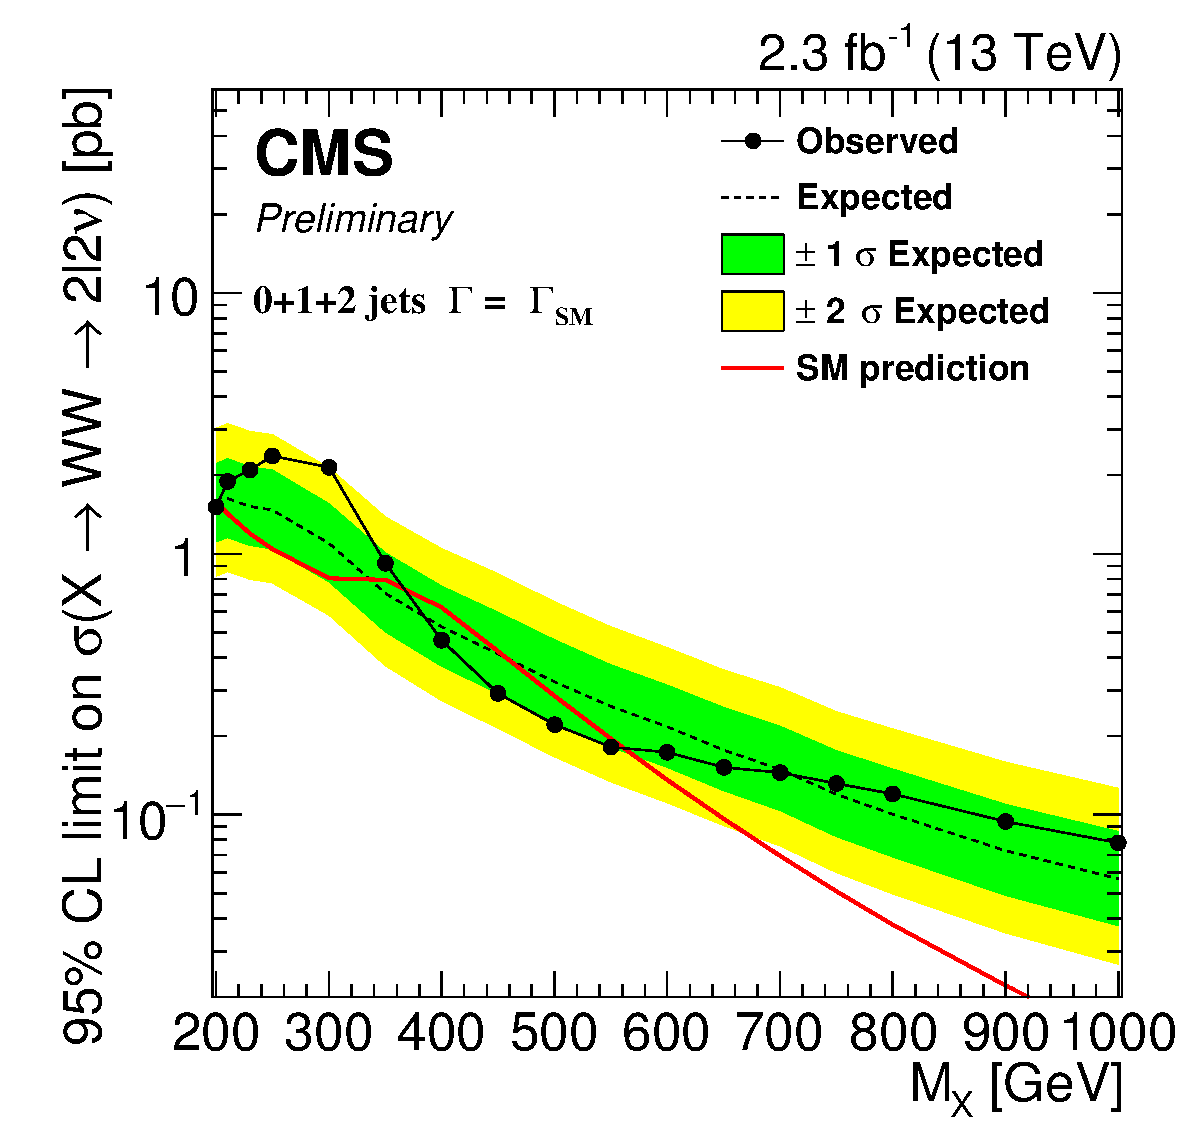
\includegraphics[width=0.45\textwidth]{images/13TeV/HighMass/limit_GSM_SMprediction.pdf}
}
\caption{
    Expected and observed exclusion limits at 95\% CL on $\sigma\times\mathcal{B}$ for the combination of the three jet categories as a function of the resonance mass. The black dotted line corresponds to the observed value while the yellow and green bands represent the $\pm 1 \sigma$ and $\pm 2 \sigma$ uncertainties respectively. Limits are displayed for four decay width hypotheses. In the case of $\Gamma' = \Gamma_{\rm SM}$ the cross section prediction is displayed as a red line.}
    \label{fig:13TeVcombobslim}
\end{figure}


